% vim: set textwidth=78 autoindent:

\section{Integración de GRASS GIS}\label{sec:grass}\index{GRASS}

% when the revision of a section has been finalized, 
% comment out the following line:
%\updatedisclaimer

El complemento de GRASS proporciona acceso a los conjuntos de datos y las funcionalidades de GRASS GIS~\cite{GRASSweb}.
Esto incluye la visualización de capas ráster y vectoriales, digitalización de capas vectoriales, edición de atributos
de vectoriales, crear nuevas capas vectoriales y análisis de datos 2D y 3D de GRASS con más de 300 módulos de GRASS.

En esta sección presentaremos las funcionalidades del complemento y daremos algunos ejemplos sobre la organización 
y trabajo con datos de GRASS. A continuación se proporcionan las principales funciones con el menú de la barra de 
herramientas, cuando inicia el complemento de GRASS, como se describe en la Sección~\ref{sec:starting_grass}:
 
\begin{itemize}
\item \toolbtntwo{grass_open_mapset}{Abrir directorio de mapas}
\item \toolbtntwo{grass_new_mapset}{Nuevo directorio de mapas}
\item \toolbtntwo{grass_close_mapset}{Cerrar directorio de mapas}
\item \toolbtntwo{grass_add_vector}{Añadir capa vectorial de GRASS}
\item \toolbtntwo{grass_add_raster}{Añadir capa ráster de GRASS}
\item \toolbtntwo{grass_new_vector_layer}{Crear nuevo vectorial de GRASS}
\item \toolbtntwo{grass_edit}{Editar capa vectorial de GRASS}
\item \toolbtntwo{grass_tools}{Abrir herramientas de GRASS}
%\item \toolbtntwo{grass_shell}{Open GRASS Shell}
\item \toolbtntwo{grass_region}{Visualizar la región actual de GRASS} 
\item \toolbtntwo{grass_region_edit}{Editar la región actual de GRASS}
\end{itemize}

\subsection{Iniciar el complemento de GRASS}\label{sec:starting_grass}
\index{GRASS!starting QGIS}

Para usar las funciones de GRASS y/o visualizar capas vectoriales o ráster de GRASS en QGIS, debe seleccionar y cargar 
el complemento de GRASS con el administrador de complementos. 
A continuacion pulse el menú 
\mainmenuopt{Complementos} > \mainmenuopt{Administrar complementos}, 
seleccione \dropmenuopt{GRASS} y pulse \button{Aceptar}. 

Ahora puede comenzar a cargar capas ráster y vectoriales desde una  
\filename{LOCALIZACIÓN} existente de 
GRASS (ver Sección \ref{sec:load_grassdata}). O puede crear una \filename{LOCALIZACIÓN} nueva con QGIS (ver Sección \ref{sec:create_loc}) 
e importar algunos datos ráster y vectoriales (ver Sección \ref{sec:import_loc_data}) 
para análisis posteriores con la
caja de herramientas de GRASS (ver Sección \ref{subsec:grass_toolbox}).

\subsection{Cargar capas ráster y vectoriales de GRASS}\label{sec:load_grassdata}\index{GRASS!loading data}

Con el complemento de GRASS, puede cargar capas vectoriales o ráster usando los botones adecuados de la barra de herramientas. 
Como ejemplo usaremos el conjunto de datos de QGIS de alaska
(ver Sección \ref{label_sampledata}), que incluye una pequeña \filename{LOCALIZACIÓN} de ejemplo con 3 capas vectoriales y 1 mapa ráster de elevación.

\begin{enumerate}
  \item Cree una carpeta nueva \filename{grassdata}, descargue el conjunto de datos de QGIS de alaska \filename{qgis\_sample\_data.zip} desde
  \url{http://download.osgeo.org/qgis/data/} y descomprima el archivo en
  \filename{grassdata}. 
  \item Inicie QGIS.
  \item Si no la ha hecho ya en una sesión anterior de QGIS, cargue el complemento de GRASS pinchando en \mainmenuopt{Complementos} > \mainmenuopt{Administrar complementos} y
  seleccionando \dropmenuopt{GRASS}. Aparecerá la barra de herramientas de GRASS en el menú de barras de herramientas.
  \item En la barra de herramientas de GRASS, pulse el icono \toolbtntwo{grass_open_mapset}{Abrir directorio de mapas} para iniciar el asistente  \filename{DIRECTORIO DE MAPAS}.
  \item Para \filename{Gisdbase} explore y seleccione o introduzca la ruta a la carpeta recién creada \filename{grassdata}.
  \item Ahora debería poder seleccionar la \filename{LOCALIZACIÓN alaska}
  y el DIRECTORIO DE MAPAS \filename{demo}. 
  \item Pulse \button{Aceptar}. Note como algunas de las herramientas de la barra de herramientas de GRASS que estaban desactivadas ahora están activadas.
  \item Pulse en \toolbtntwo{grass_add_raster}{Añadir capa ráster de GRASS}, seleccione el mapa llamado \filename{gtopo30} y pulse \button{Aceptar}. Se visualizará la capa de elevaciones.
  \item Pulse en \toolbtntwo{grass_add_vector}{Añadir capa vectorial de GRASS},
  seleccione el mapa \filename{alaska} y pulse \button{Aceptar}. La capa con el contorno de Alaska se superpondrá sobre el mapa gtopo30. Ahora puede adaptar las propiedades de la capa como se describe en el capítulo \ref{sec:vectorprops}, por ejemplo, cambiar la opacidad o el color de relleno o de línea exterior.
  \item Cargue también las otras dos capas vectoriales \filename{rivers} y
  \filename{airports} y adapte sus propiedades.
\end{enumerate}

Como puede ver, es muy sencillo cargar capas ráster y vectoriales de GRASS en QGIS. Vea las siguientes secciones para editar 
datos de GRASS y crear nuevas \filename{LOCALIZACIONES}. Hay más \filename{LOCALIZACIONES} de 
muestra disponibles en la web de GRASS en \url{http://grass.osgeo.org/download/data.php}.

\begin{Tip}\caption{\textsc{Cargar datos de GRASS}}
\qgistip{Si tiene problemas para cargar datos o QGIS termina de forma anormal, asegúrese de que ha cargado el complemento de GRASS correctamente como se describe en la Sección \ref{sec:starting_grass}.
}
\end{Tip} 

\subsection{LOCALIZACIÓN Y DIRECTORIO DE MAPAS DE GRASS}\label{sec:about_loc}

Los datos de GRASS se guardan en un directorio denominado GISDBASE. Este directorio, 
a menudo llamado \filename{grassdata}, 
se debe crear antes de empezar a trabajar con el complemento de GRASS en QGIS. Dentro de ese directorio, los datos SIG de GRASS están
organizados por proyectos guardados en subdirectorios llamados \filename{LOCALIZACIÓN}. 
Cada \filename{LOCALIZACIÓN} se define 
por su sistema de coordenadas, proyección del mapa y límites geográficos. Cada \filename{LOCALIZACIÓN} puede tener 
varios \filename{DIRECTORIOS DE MAPAS} (subdirectorios de la \filename{LOCALIZACIÓN}) que se usan para subdividir el proyecto 
en diferentes temas, subregiones o entornos de trabajo para distintos miembros de un equipo de trabajo (Neteler \& Mitasova 2008 
\cite{neteler_mitasova08}). Para poder analizar capas vectoriales y ráster con los módulos de GRASS, debe importarlos a una \filename{LOCALIZACIÓN} de GRASS.
\footnote{Esto no es estrictamente cierto - con los módulos de GRASS 
\filename{r.external} y \filename{v.external} puede crear enlaces de sólo lectura a conjuntos de datos externos admitidos por 
GDAL/OGR sin importarlos. Pero como esta no es la forma habitual de empezar a trabajar con GRASS para principiantes, esta funcionalidad no se describirá aquí.}

\begin{figure}[ht]
\begin{center}
\caption{Datos de GRASS en la LOCALIZACIÓN alaska (adaptado de Neteler \& 
Mitasova 2008 \cite{neteler_mitasova08})}\label{fig:grass_location}\smallskip

\includegraphics[clip=true]{grass_location}
\end{center}  
\end{figure}

\subsubsection{Crear una nueva LOCALIZACIÓN de GRASS}\label{sec:create_loc}

Como ejemplo mostramos las instrucciones de cómo se creó la \filename{LOCALIZACIÓN Alaska} de GRASS,
que está en la proyección Albers Equal Area, para el conjunto de datos de muestra de QGIS. Esta
\filename{LOCALIZACIÓN Alaska} de GRASS se usará para todos los ejemplos y ejercicios en los siguientes capítulos
relacionados con GRASS GIS. Es útil descargar e instalar el conjunto de datos en su ordenador \ref{label_sampledata}).

\begin{figure}[ht]
\begin{center}
\caption{Crear una nueva LOCALIZACIÓN de GRASS o un nuevo DIRECTORIO DE MAPAS en QGIS \nixcaption}
\label{fig:create_grass_location}\smallskip
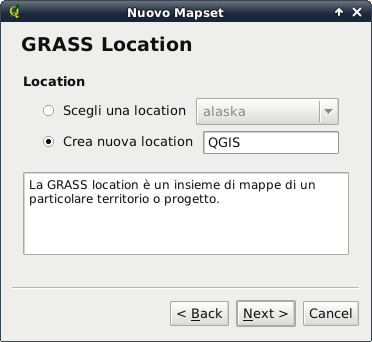
\includegraphics[clip=true, width=10cm]{create_grass_location}
\end{center}  
\end{figure}

\begin{enumerate}
  \item Inicie QGIS y asegúrese de que el complemento de GRASS está cargado.
  \item Visualice el archivo shape \filename{alaska.shp} (ver Sección
  \ref{sec:load_shapefile}) del conjunto de datos alaska de QGIS~\ref{label_sampledata}.
  \item En la barra de herramientas de GRASS, pulse en el icono \toolbtntwo{grass_open_mapset}{abrir
    directorio de mapas} para llamar al asistente \filename{DIRECTORIO DE MAPAS}.
  \item Seleccione una carpeta de base de datos de GRASS (GISDBASE) existente 
  \filename{grassdata} o cree una para la nueva \filename{LOCALIZACIÓN} usando un administrador de archivos 
  de su ordenador. Pulse luego \button{Siguiente}. 
  \item Podemos usar el asistente para crear un nuevo \filename{DIRECTORIO DE MAPAS} dentro de una 
   \filename{LOCALIZACIÓN} existente (ver Sección~\ref{sec:add_mapset}) o para crear 
  una nueva \filename{LOCALIZACIÓN} todo junto. Marque el botón circular
  \radiobuttonon{Crear nueva localización} (ver Imagen \ref{fig:create_grass_location}).
  \item Introduzca un nombre para la \filename{LOCALIZACIÓN} - nosotros usamos alaska - y pulse 
  \button{Siguiente} 
  \item Defina la proyección pulsando el botón circular
  \radiobuttonon{Proyección} para activar la lista de proyecciones.
  \item Estamos usando la proyección Albers Equal Area Alaska (pies). Como sabemos que está representada por el EPSG ID 2964, lo introducimos 
  en la casilla de búsqueda. (Nota: Si quiere repetir este proceso para otra 
  \filename{LOCALIZACIÓN} y proyección y no ha memorizado el EPSG ID, 
  pulse en el icono
  \toolbtntwo{mIconProjectionEnabled}{proyector} en la esquina inferior derecha de la barra de estado (ver Sección \ref{label_projstart})).
  \item Pulse \button{Encontrar} para seleccionar la proyección.
  \item Pulse \button{Siguiente} 
  \item Para definir la región predeterminada, tenemos que introducir los límites de la \filename{LOCALIZACIÓN} en dirección Norte, Sur, Este y Oeste. 
  Aquí simplemente pulsaremos el botón \button{Establecer la extensión actual de QGIS}, para aplicar la extensión de la  
  capa cargada \filename{alaska.shp} como extensión de la región predeterminada de GRASS.
  \item Pulse \button{Siguiente} 
  \item También tenemos que definir un \filename{DIRECTORIO DE MAPAS} dentro de nuestra nueva 
  \filename{LOCALIZACIÓN}. Póngale el nombre que prefiera - nosotros usamos demo.
  \footnote{Cuando se crea una nueva \filename{LOCALIZACIÓN}, GRASS automáticamente 
  crea un \filename{DIRECTORIO DE MAPAS} especial llamado \filename{PERMANENT} diseñado para 
  guardar los datos básicos del proyecto, su extensión espacial predeterminada y 
  la deficición del sistema de coordenadas (Neteler \& Mitasova 2008 
  \cite{neteler_mitasova08}).}
  \item Compruebe el resumen para asegurarse que es correcto y pulse
  \button{Terminar} 
  \item Se creará la nueva \filename{LOCALIZACIÓN alaska} y dos \filename{DIRECTORIOS DE MAPAS demo}
  y \filename{PERMANENT}. El conjunto de trabajo abierto actual es el
  \filename{DIRECTORIO DE MAPAS demo}, como lo ha definido.
  \item Vea como algunas de las herramientas de la barra de herramientas de GRASS que estaban desactivadas ahora están activadas.
\end{enumerate}

Si le parecieron muchos pasos, ésto no es tan malo y sí una forma muy rápida de crear una \filename{LOCALIZACIÓN}. La \filename{LOCALIZACIÓN alaska} ahora está lista para importar datos (ver Sección \ref{sec:import_loc_data}).
También puede usar los datos vectoriales y ráster ya existentes en la \filename{LOCALIZACIÓN alaska} de muestra incluida en el conjunto de datos de Alaska de QGIS 
\ref{label_sampledata} e ir a la Sección \ref{label_vectmodel}.

\subsubsection{Añadir un nuevo DIRECTORIO DE MAPAS}\label{sec:add_mapset}

Un usuario sólo tiene permiso de escritura en el \filename{DIRECTORIO DE MAPAS} de GRASS que ha creado. Esto 
significa, además de acceder a su propio \filename{DIRECTORIO DE MAPAS}, cada usuario también puede leer mapas en los 
\filename{DIRECTORIOS DE MAPAS} de otros usuarios, pero sólo puede modificar o eliminar los mapas de su propio 
\filename{DIRECTORIO DE MAPAS}. Todos los \filename{DIRECTORIOS DE MAPAS} incluyen un archivo 
\filename{WIND} que guarda los valores de coordenadas del contorno actual y 
la resolución ráster actualmente seleccionada (Neteler \& Mitasova 2008 
\cite{neteler_mitasova08}, ver Sección \ref{sec:grass_region}). 

\begin{enumerate}
  \item Inicie QGIS y asegúrese de que el complemento de GRASS está cargado.
  \item En la barra de herramientas de GRASS, pulse en el icono 
  \toolbtntwo{grass_new_mapset}{Nuevo directorio de mapas} para lanzar el asistente
  \filename{DIRECTORIO DE MAPAS}.
  \item Seleccione la carpeta de la base de datos de GRASS (GISDBASE) \filename{grassdata} 
  con la \filename{LOCALIZACIÓN alaska}, donde queremos añadir un nuevo 
  \filename{DIRECTORIO DE MAPAS}, llamado test.
  \item Pulse \button{Siguiente}. 
  \item Podemos usar este asistente para crear un nuevo \filename{DIRECTORIO DE MAPAS} dentro de 
  una \filename{LOCALIZACIÓN} existente o crear una nueva \filename{LOCALIZACIÓN} 
  todo a la vez. Pulse el botón circular
  \radiobuttonon{Seleccionar localización} 
  (ver Imagen \ref{fig:create_grass_location}) y pulse \button{Siguiente}.
  \item Introduzca el nombre \filename{text} para el nuevo \filename{DIRECTORIO DE MAPAS}. En la parte de abajo 
  del asistente verá una lista de \filename{DIRECTORIOS DE MAPAS} existente y sus propietarios.
  \item Pulse \button{Siguiente}, compruebe el resumen para asegurarse de que todo está correcto y pulse \button{Finalizar}.
\end{enumerate}

\subsection{Importar datos a una LOCALIZACIÓN de GRASS}\label{sec:import_loc_data}

Esta Sección da un ejemplo de cómo importar datos ráster y vectoriales a la 
\filename{LOCALIZACIÓN} 
\filename{alaska} de GRASS proporcionada por el conjunto de datos alaska de QGIS. Por lo tanto usaremos un mapa ráster de cobertura
del terreno \filename{landcover.img} y un archivo vectorial GML \filename{lakes.gml} del conjunto de datos alaska de QGIS \ref{label_sampledata}.

\begin{enumerate}
  \item Inicie QGIS y asegúrese de que el complemento de GRASS está cargado.
  \item En la barra de herramientas de GRASS, pulse en el icono 
  \toolbtntwo{grass_open_mapset}{Abrir directorio de mapas} para lanzar el asistente
  \filename{DIRECTORIO DE MAPAS}.
  \item Seleccione como base de datos de GRASS la carpeta \filename{grassdata} del conjunto 
  de datos alaska de QGIS, la \filename{LOCALIZACIÓN alaska}, y el \filename{DIRECTORIO DE MAPAS} 
  \filename{demo} y pulse \button{Aceptar}.
  \item Ahora pulse el icono \toolbtntwo{grass_tools}{Abrir herramientas de GRASS}. Aparecerá la caja de herramientas de 
  GRASS (ver Sección \ref{subsec:grass_toolbox}).
  \item Para importar el mapa ráster \filename{landcover.img}, pulse en el módulo 
  \filename{r.in.gdal} en la pestaña 
  \tab{Árbol de módulos}. Este módulo de GRASS le permite importar archivos ráster admitidos por GDAL a una 
  \filename{LOCALIZACIÓN} de GRASS. Aparecerá el diálogo del módulo para \filename{r.in.gdal}.
  \item Navegue a la carpeta \filename{raster} en el conjunto de datos alaska de QGIS y seleccione el archivo \filename{landcover.img}.
  \item Como nombre del ráster de salida defina \filename{landcover\_grass} y pulse 
  \button{Ejecutar}. En la pestaña \tab{Salida} se ve la orden de GRASS que se está ejecutando actualmente 
  \filename{r.in.gdal -o input=/path/to/landcover.img 
  output=landcover\_grass}.
  \item Cuando diga \textbf{Terminado con éxito} pulse \button{Ver salida}. 
  La capa ráster \filename{landcover\_grass} ahora está importada a GRASS y se visualizará en el lienzo de QGIS.
  \item Para importar el archivo GML vectorial \filename{lakes.gml}, pulse el módulo 
  \filename{v.in.ogr} en la pestaña \tab{Árbol de módulos}. Este módulo de GRASS permite importar archivos vectoriales admitidos 
  por OGR a una \filename{LOCALIZACIÓN} de GRASS. Aparecerá el dialogo del módulo para
  \filename{v.in.ogr}.
  \item Navegue a la carpeta \filename{gml} del conjunto de datos alaska de QGIS y seleccione el archivo \filename{lakes.gml} como archivo OGR.
  \item Como nombre del vectorial de salida defina \filename{lakes\_grass} y pulse 
  \button{Ejecutar}. No tiene que preocuparse 
  de las otras opciones en este ejemplo. En la pestaña \tab{Salida} se ve la instrucción de GRASS que se está ejecutando
  \filename{v.in.ogr -o dsn=/path/to/lakes.gml output=lakes\_grass}.
  \item Cuando diga \textbf{Terminado con éxito} pulse \button{Ver salida}. 
  La capa vectorial \filename{lakes\_grass} ahora está importa a GRASS y se visualizará en el lienzo de QGIS.
\end{enumerate}


\subsection{El modelo de datos vectoriales de GRASS}\label{label_vectmodel}\index{GRASS!vector data
model}

Es importante entender el modelo de datos vectoriales de GRASS antes de digitalizar.\index{GRASS!digitizing} En general, GRASS usa un modelo vectorial topológico.\index{GRASS!topology} Esto significa que las áreas no se representan como polígonos cerrados, sino por uno o más contornos. Esto significa que las áreas no se representan como polígonos cerrados, sino por uno o más contornos.
Los contornos deben estar conectados sin saltos. Un área es identificada (etiquetada) por los centroides del área.

Además de contornos y centroides, un mapa vectorial puede contener puntos y líneas. Todos estos elementos geométricos 
pueden estar mezclados en un vectorial y se representarán en diferentes «capas» dentro de un mapa vectorial de GRASS.
Así, en GRASS una capa no es un mapa vectorial o ráster, sino un nivel dentro de un mapa vectorial. Es importante distinguir esto claramente.
\footnote{Aunque es posible mezclar elementos de distinta geometría, no es habitual e incluso en GRASS sólo se usa en casos especiales
tales como el análisis de redes vectoriales. Normalmente es preferible guardar elementos de distinta geometría en diferentes capas.}

Es posible guardar más «capas» en un conjunto de datos vectorial. Por ejemplo, se pueden guardar campos, bosques y lagos en un vectorial.
Los bosques y lagos adyacentes pueden compartir el mismo contorno, pero tiene tablas de atributos separadas. También es posible
adjuntar atributos a los contornos. Por ejemplo, el contorno entre lago y bosque es una carretera, por lo que puede tener una tabla de atributos diferente.
 
La «capa» de los objetos espaciales se define por la «capa» dentro de GRASS. «Capa» es un número que define si hay más de 
una capa dentro del conjunto de datos, por ejemplo, si la geometría es bosque o lago. De momento, puede ser sólo un número, 
en el futuro GRASS también admitirá nombres como campos en la interfaz de usuario.

Los atributos se pueden guardar dentro de la \filename{LOCALIZACIÓN} de GRASS como DBase o SQLITE3 o en bases de datos externas, por ejemplo PostgreSQL, MySQL, 
Oracle, etc.\index{GRASS!attribute storage}

Los atributos en las tablas de las bases de datos se enlazan a los elementos geométricos usando un valor de «categoría».
\index{GRASS!attribute linkage} La «categoría» (clave, ID) es un entero adjunto a los primitivos de la geometría y se 
usa como el enlace a una columna de la tabla de la base de datos.

\begin{Tip}\caption{\textsc{Aprender el modelo vectorial de GRASS}}
\qgistip{
La mejor forma de aprender el modelo vectorial de GRASS y sus capacidades es descargar uno de los muchos manuales de GRASS, donde se describe el modelo vectorial con más detalle. Vea \url{http://grass.osgeo.org/gdp/manuals.php} para más información, libros y manuales en varios idiomas.
}
\end{Tip} 

\subsection{Crear una nueva capa vectorial de GRASS}\label{sec:creating_new_grass_vectors}\index{GRASS!Creating new vectors|see{editing!creating a new layer}}

Para crear una nueva capa vectorial de GRASS con el complemento de GRASS pulse el icono de la barra de herramientas 
\toolbtntwo{grass_new_vector_layer}{Crear nuevo vectorial de GRAS}. Introduzca un nombre en el cuadro de texto y puede comenzar 
a digitalizar puntos, líneas o polígonos, siguiendo el procedimiento descrito en la Sección 
\ref{grass_digitising}. 

En GRASS es posible organizar todo tipo de geometrías (puntos, líneas y áreas) en una capa, porque GRASS usa un modelo
vectorial topológico, así que no necesita seleccionar el tipo de geometría al crear un nuevo vectorial de GRASS. Esto es
diferente de la creación de archivos shape con QGIS, ya que los archivos shape utilizan el modelo vectorial de objetos 
espaciales simples (ver Sección \ref{sec:create shape}).

\begin{Tip}\caption{\textsc{Crear una tabla de atributos para una nueva capa vectorial de GRASS}}
\qgistip{
Si quiere asignar atributos a los objetos espaciales digitalizados de su geometría, asegúrese de crear una tabla de 
atributos con las columnas necesarias antes de empezar a digitalizar (ver Imagen \ref{fig:grass_digitizing_table}).
}
\end{Tip} 

\subsection{Digitalizar y editar una capa vectorial de GRASS}\index{GRASS!digitizing tools}\label{grass_digitising}

Las herramientas de digitalización para las capas vectoriales de GRASS son accesibles usando el icono \toolbtntwo{grass_edit}{Editar capa vectorial de GRASS} 
de la barra de herramientas. Asegúrese de que ha cargado un vectorial de GRASS y que éste es la capa seleccionada en 
la leyenda antes de pulsar la herramienta de edición. La figura \ref{fig:grass_digitizing_category} muestra el diálogo
de edición de GRASS que aparece cuando pulsa en la herramienta de edición. Las herramientas y configuración se describen en las siguientes secciones.

\begin{Tip}\caption{\textsc{Digitalizar polígonos en GRASS}}
\qgistip{
Si quiere crear polígonos en GRASS, primero se digitaliza el contorno del polígono, estableciendo el modo a \usertext{Sin categoría}. 
Luego se añade un centroide (punto de etiqueta) dentro del contorno cerrado, estableciendo el modo a \usertext{Siguiente no usado}. 
La razón es que un modelo vectorial topológico enlaza la información de los atributos de un polígono siempre al centroide
y no al contorno.
}
\end{Tip} 

\minisec{Barra de herramientas}\label{label_grasstoolbar}

En la Figura \ref{fig:grass_digitizing_toolbar} puede ver las herramientas de digitalización proporcionadas por el complemento de GRASS. La Tabla \ref{tab:grass_tools}
explica las funcionalidades disponibles.

\begin{figure}[h]
   \begin{center}
   \caption{Barra de herramientas de digitalización de GRASS \nixcaption}\label{fig:grass_digitizing_toolbar} 
   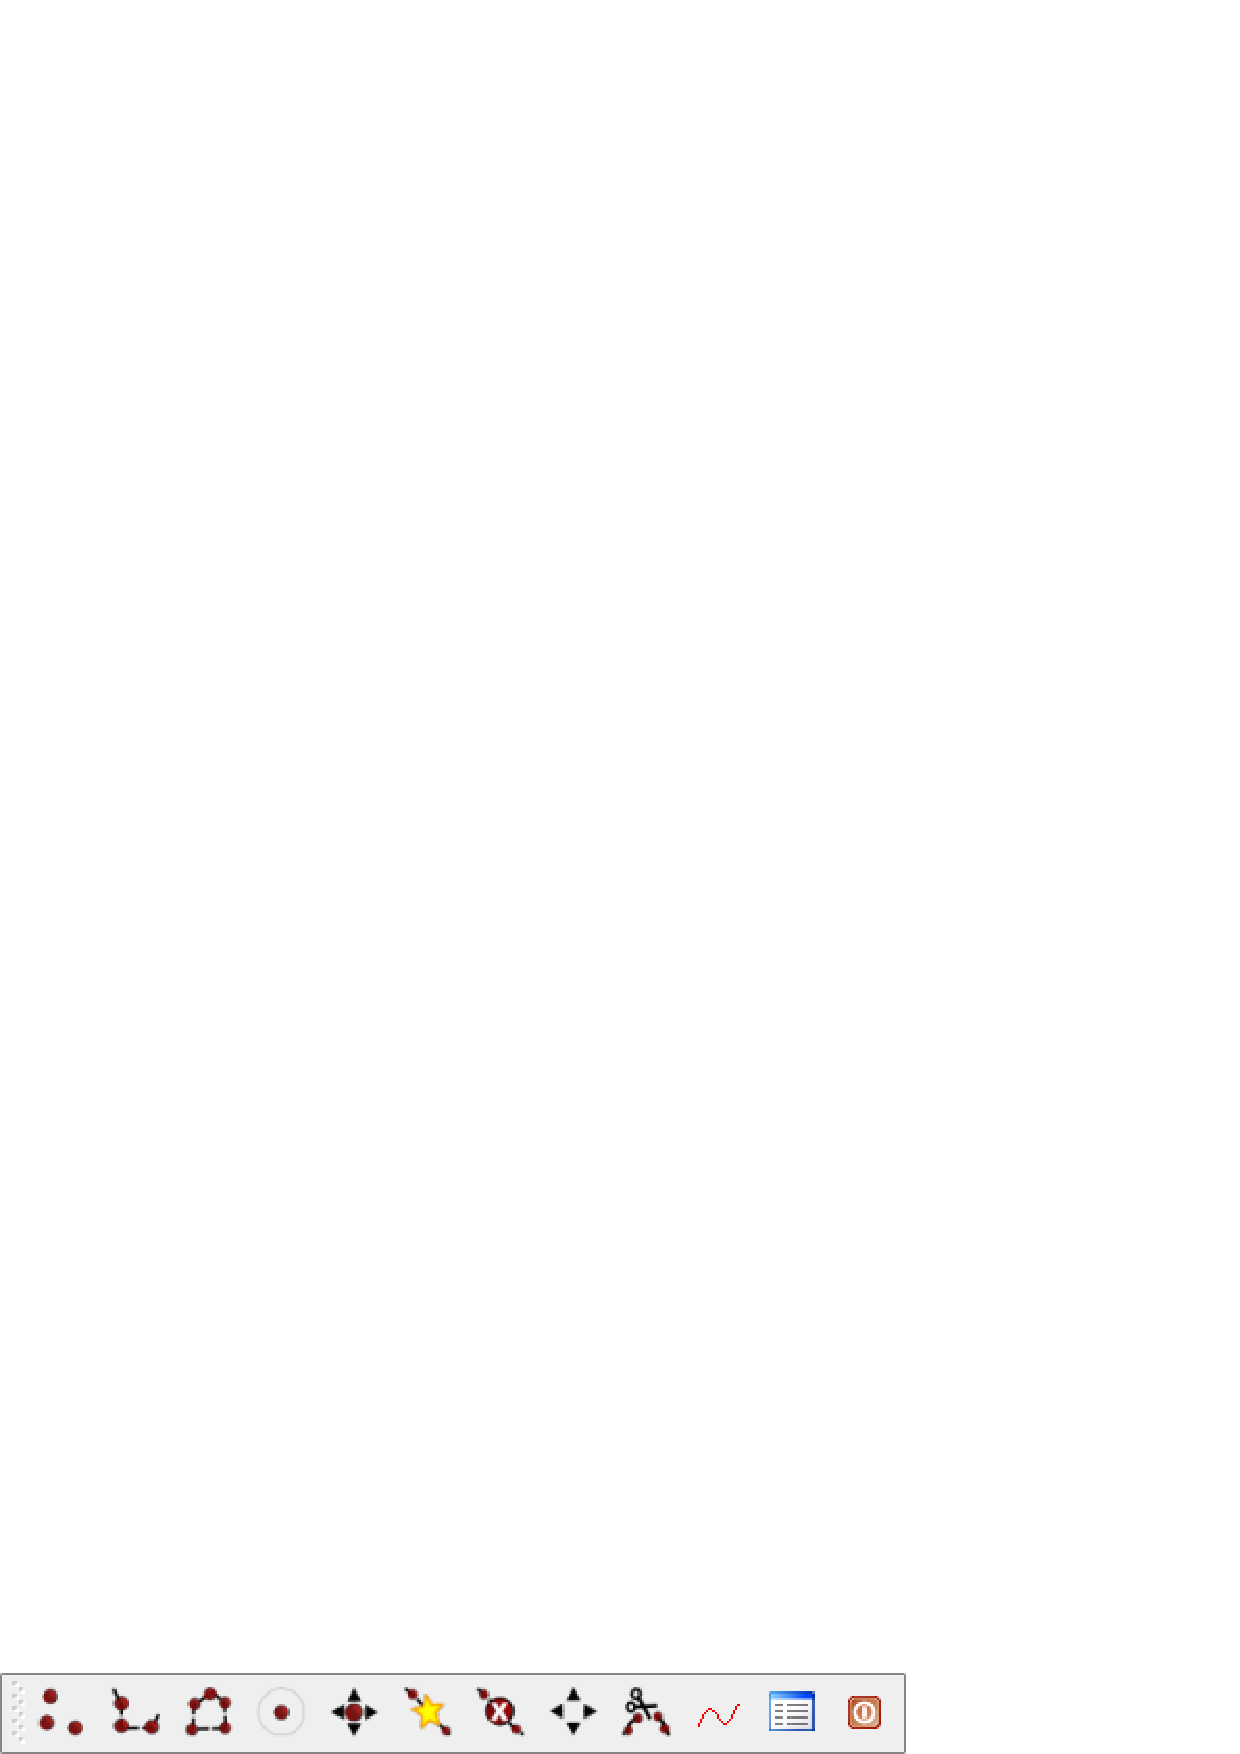
\includegraphics[clip=true,width=12cm]{grass_digitizing_toolbar}
\end{center}  
\end{figure}

\begin{table}[h]\index{GRASS!digitizing tools}
\centering
\caption{Herramientas de digitalización de GRASS}\label{tab:grass_tools}\medskip
 \begin{tabular}{|l|l|p{5in}|}
 \hline \textbf{Icono} & \textbf{Herramienta} & \textbf{Propósito} \\
\hline 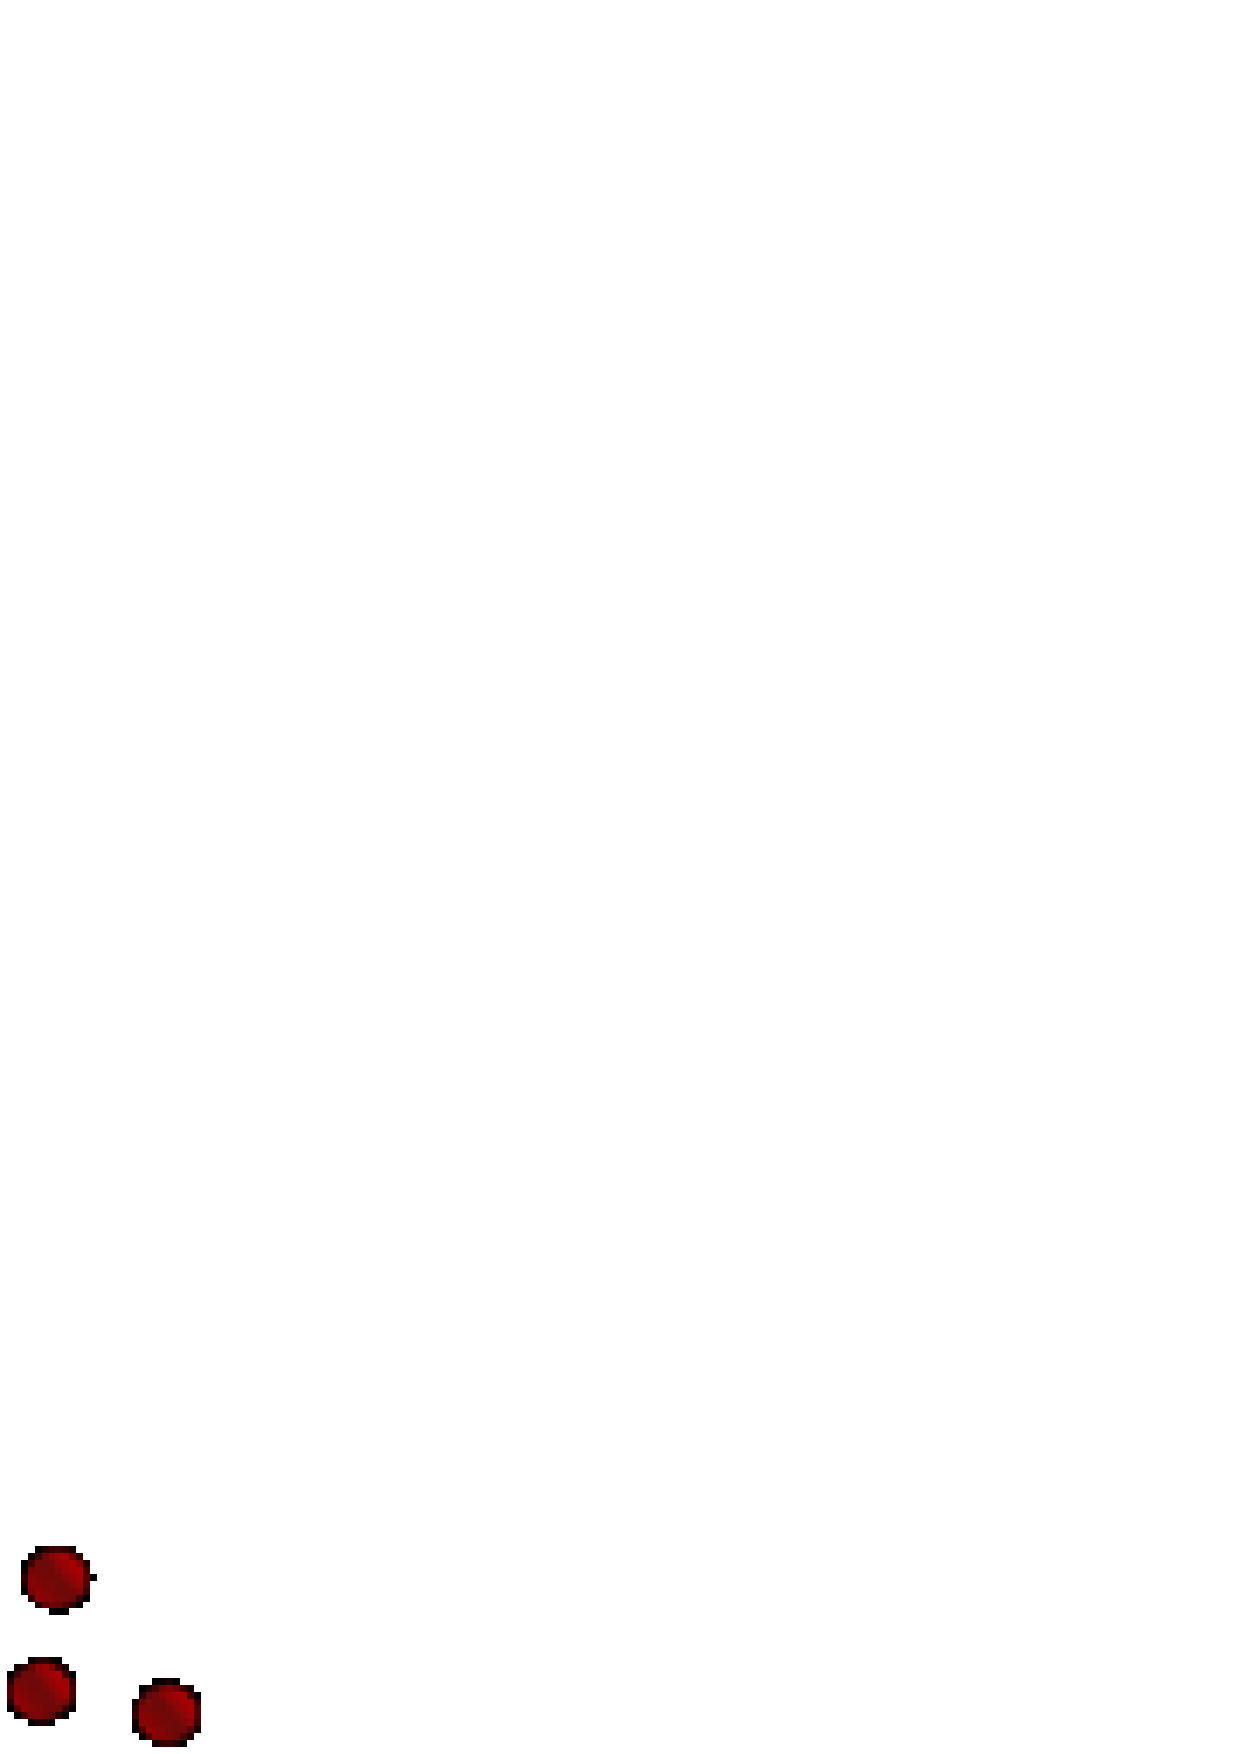
\includegraphics[width=0.7cm]{grass_new_point} & Nuevo punto & Digitalizar un punto nuevo \\
\hline 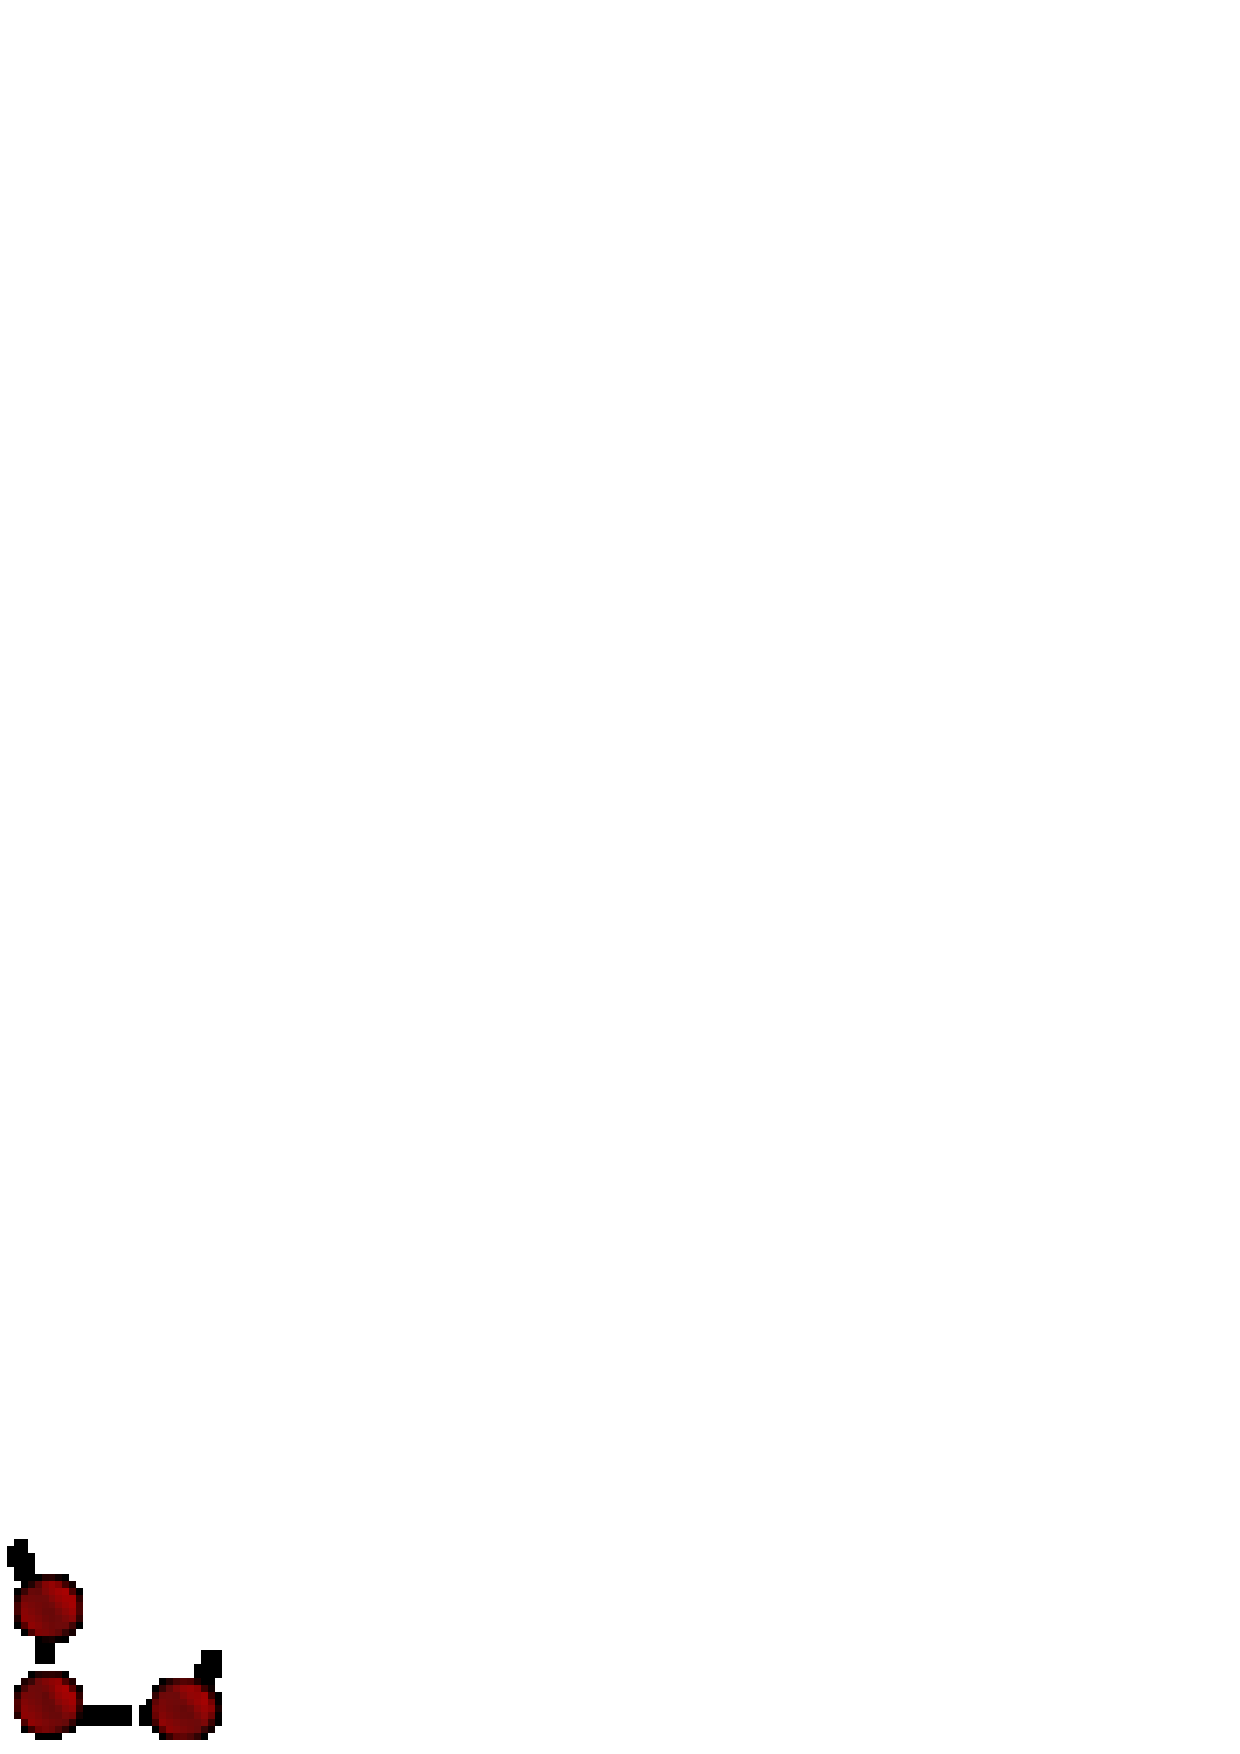
\includegraphics[width=0.7cm]{grass_new_line} & Nueva línea &  Digitalizar una línea nueva (finaliza al seleccionar una herramienta nueva) \\
\hline 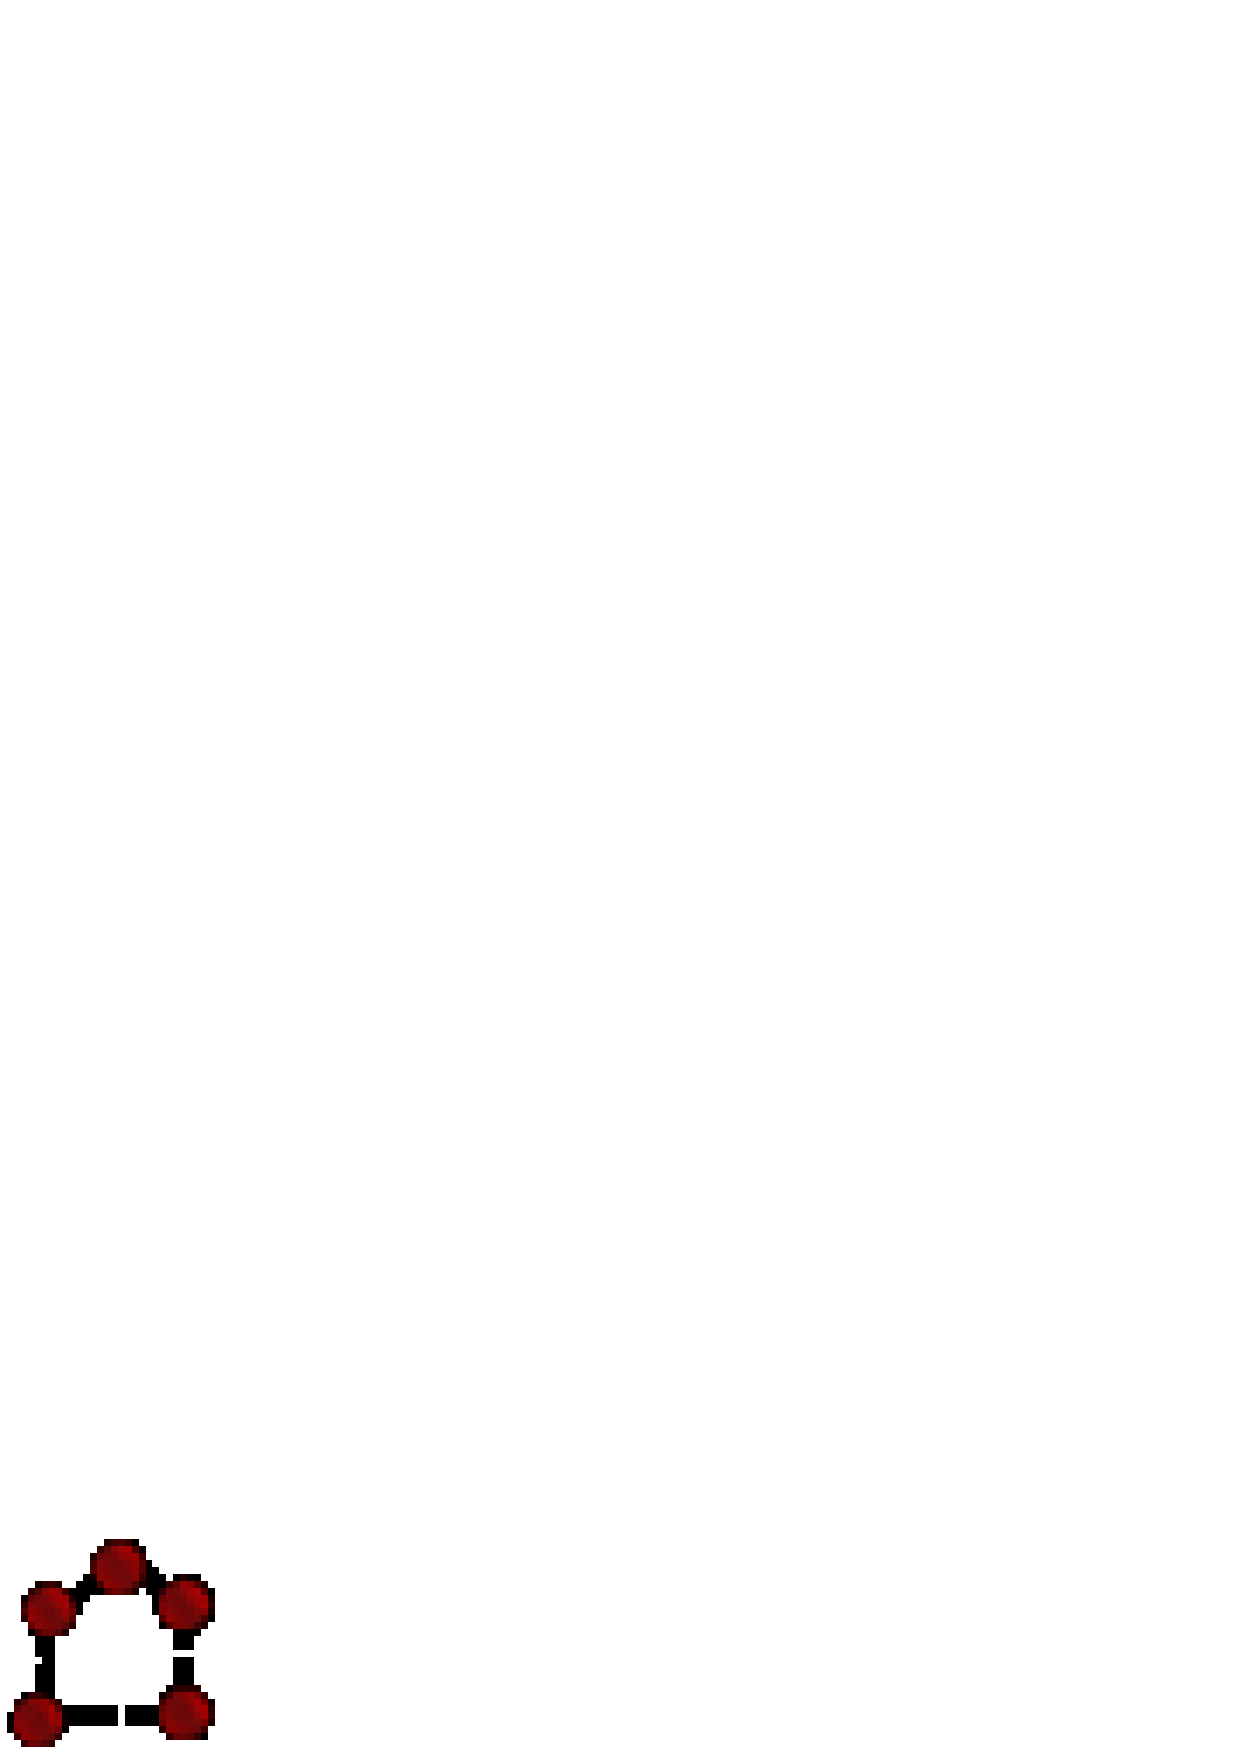
\includegraphics[width=0.7cm]{grass_new_boundary} & Nuevo contorno & Digitalizar un contorno nuevo (finaliza al seleccionar una herramienta nueva)\\
\hline 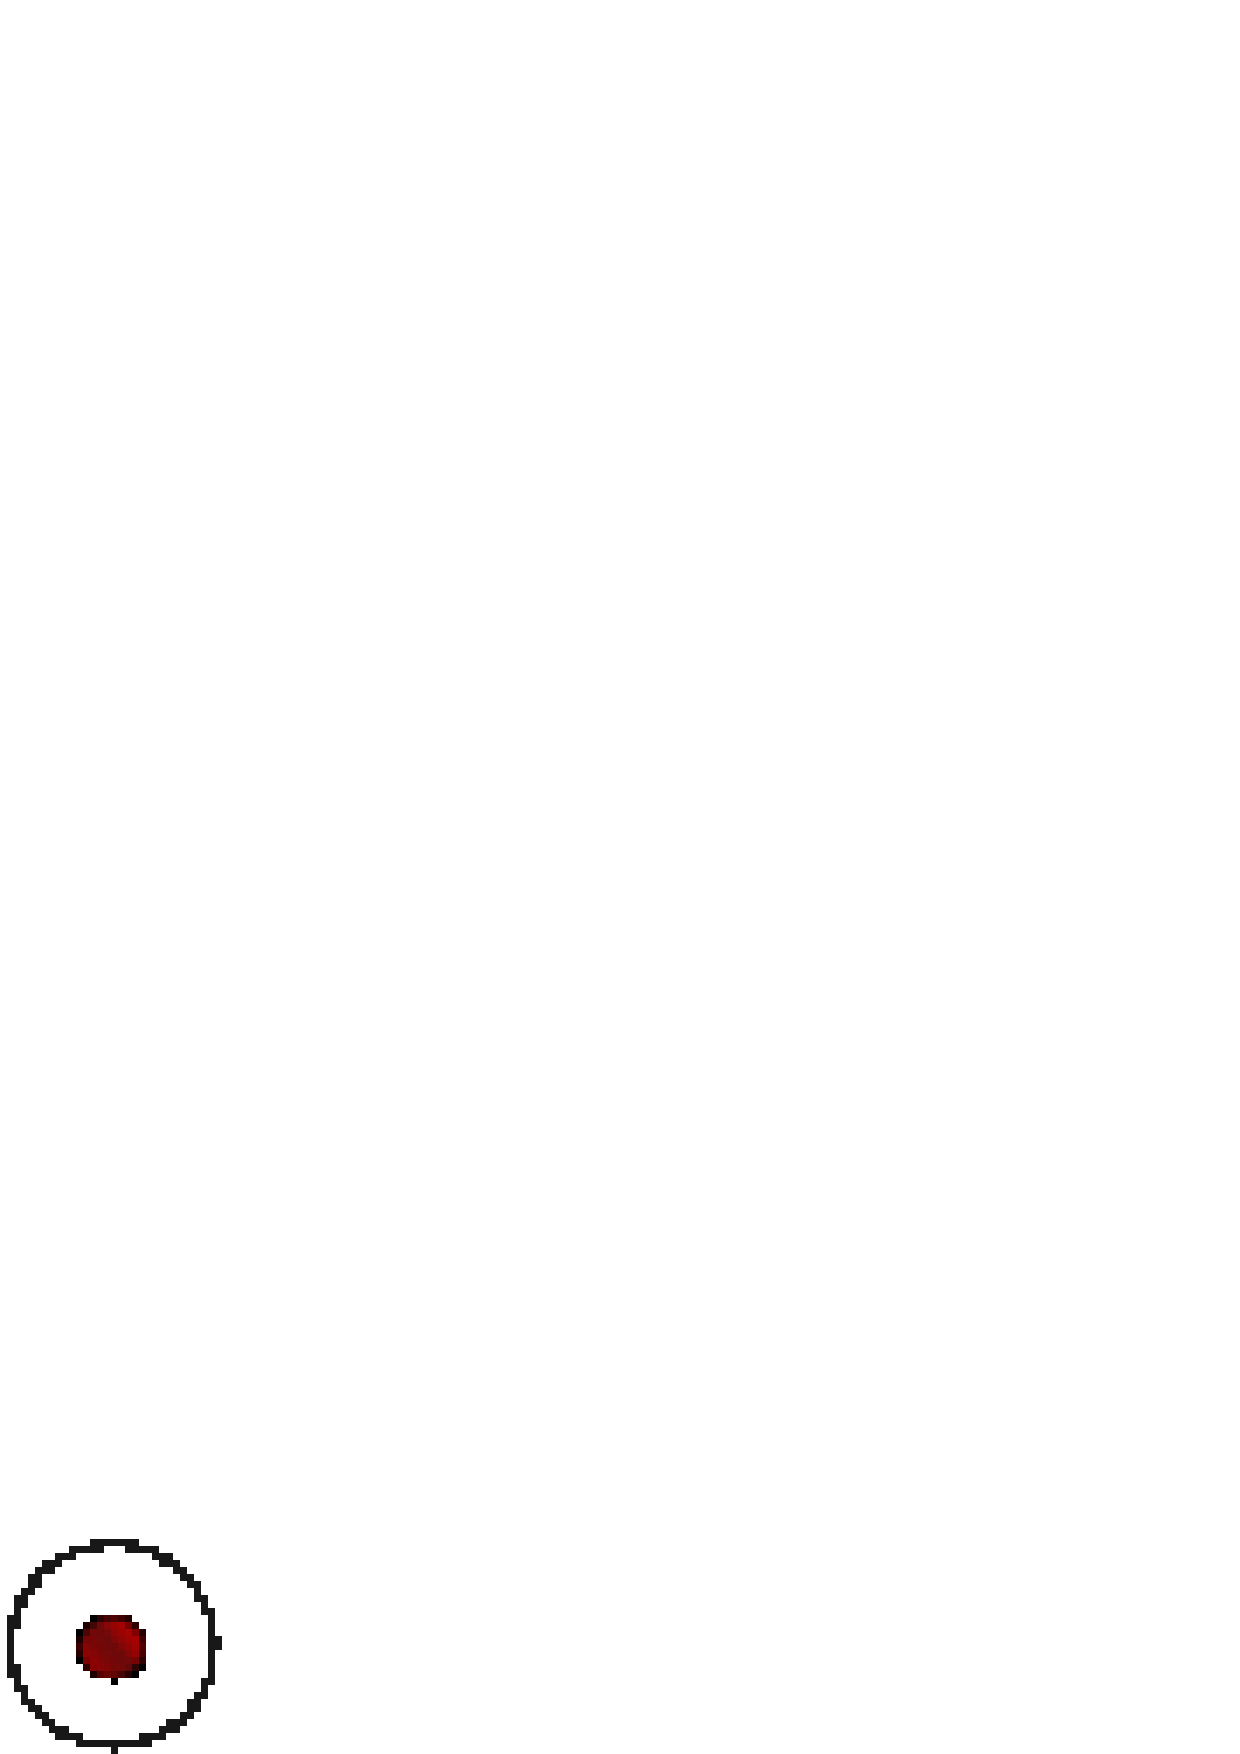
\includegraphics[width=0.7cm]{grass_new_centroid} & Nuevo centroide & Digitalizar un centroide nuevo (etiquetar un área existente)\\
\hline 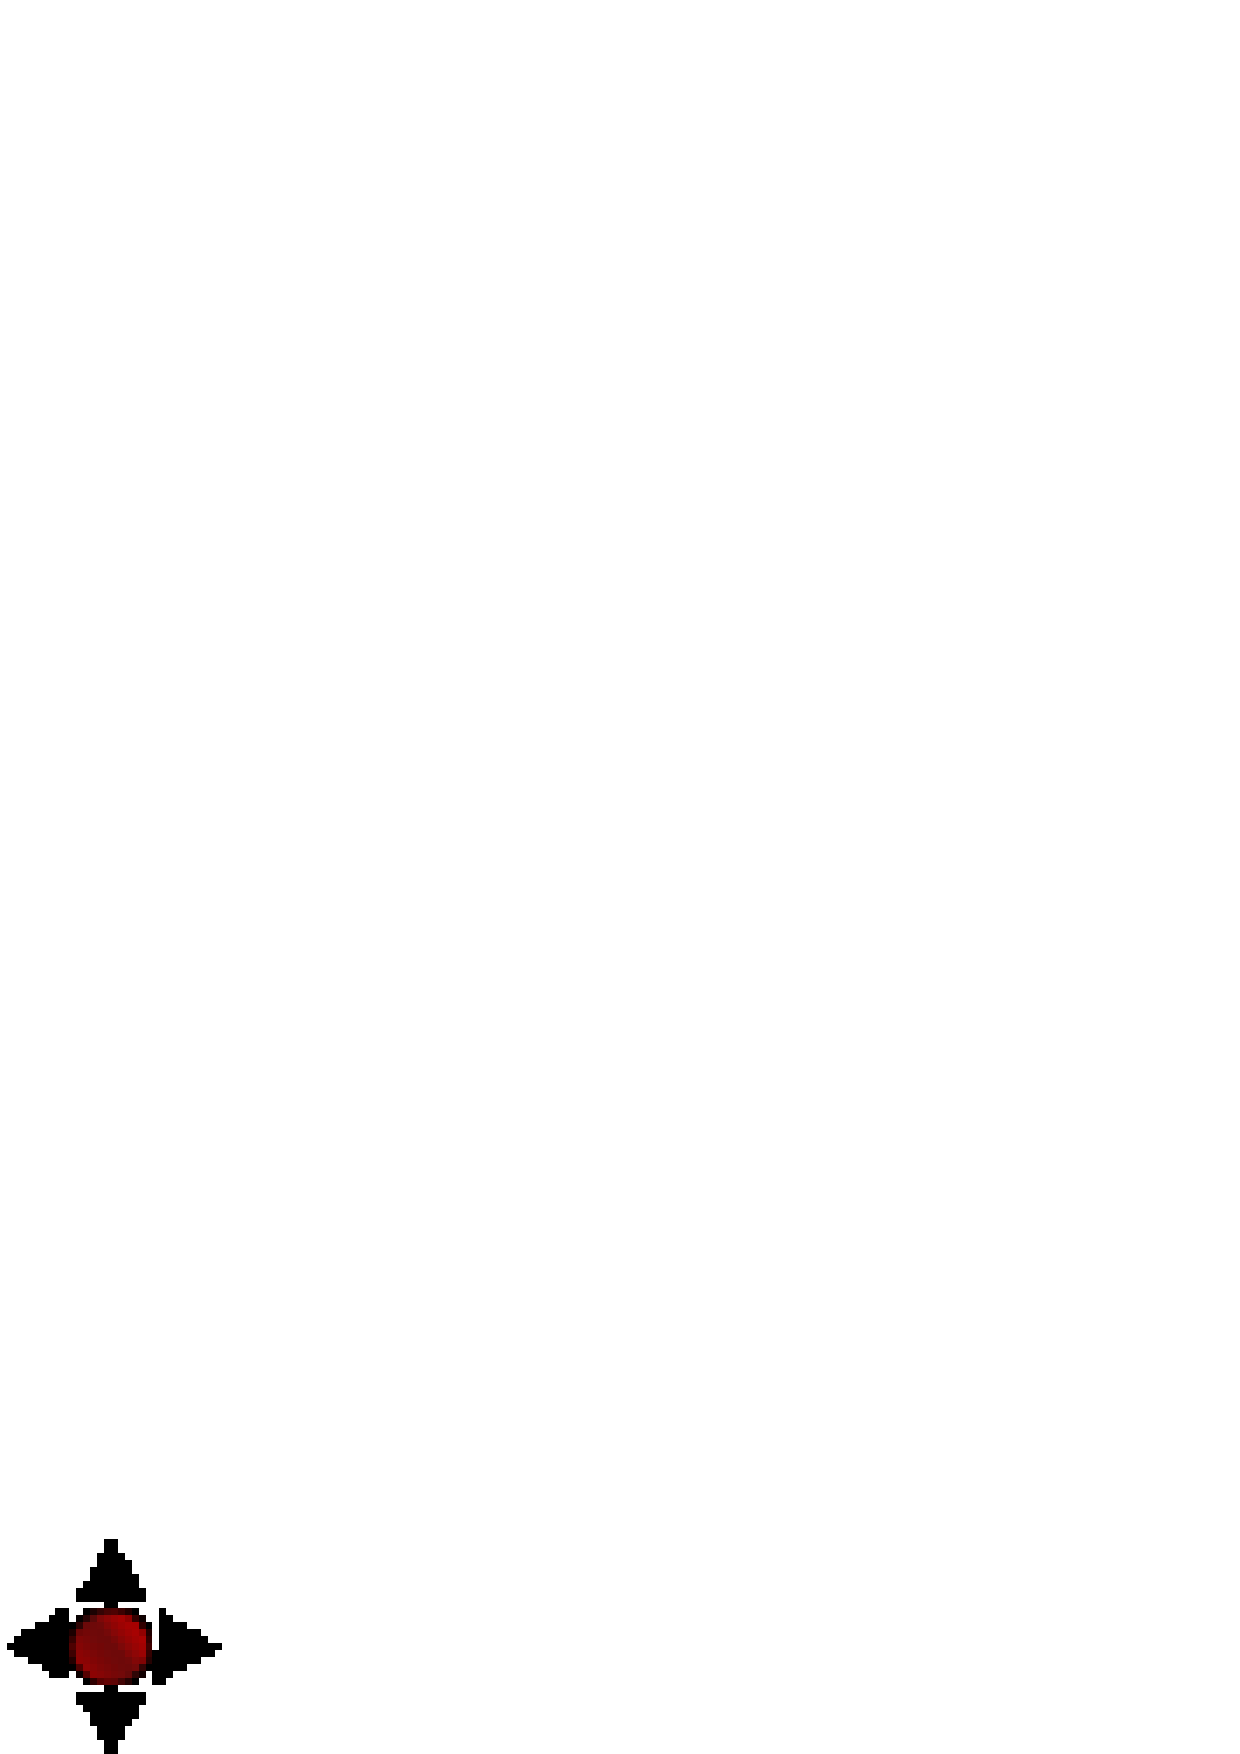
\includegraphics[width=0.7cm]{grass_move_vertex} & Mover vértice & Seleccionar un vértice de una línea o contorno existente e identificar una nueva posición\\
\hline 
\includegraphics[width=0.7cm]{grass_add_vertex} & Añadir vértice & Añadir un vértice nuevo a una línea existente\\
\hline 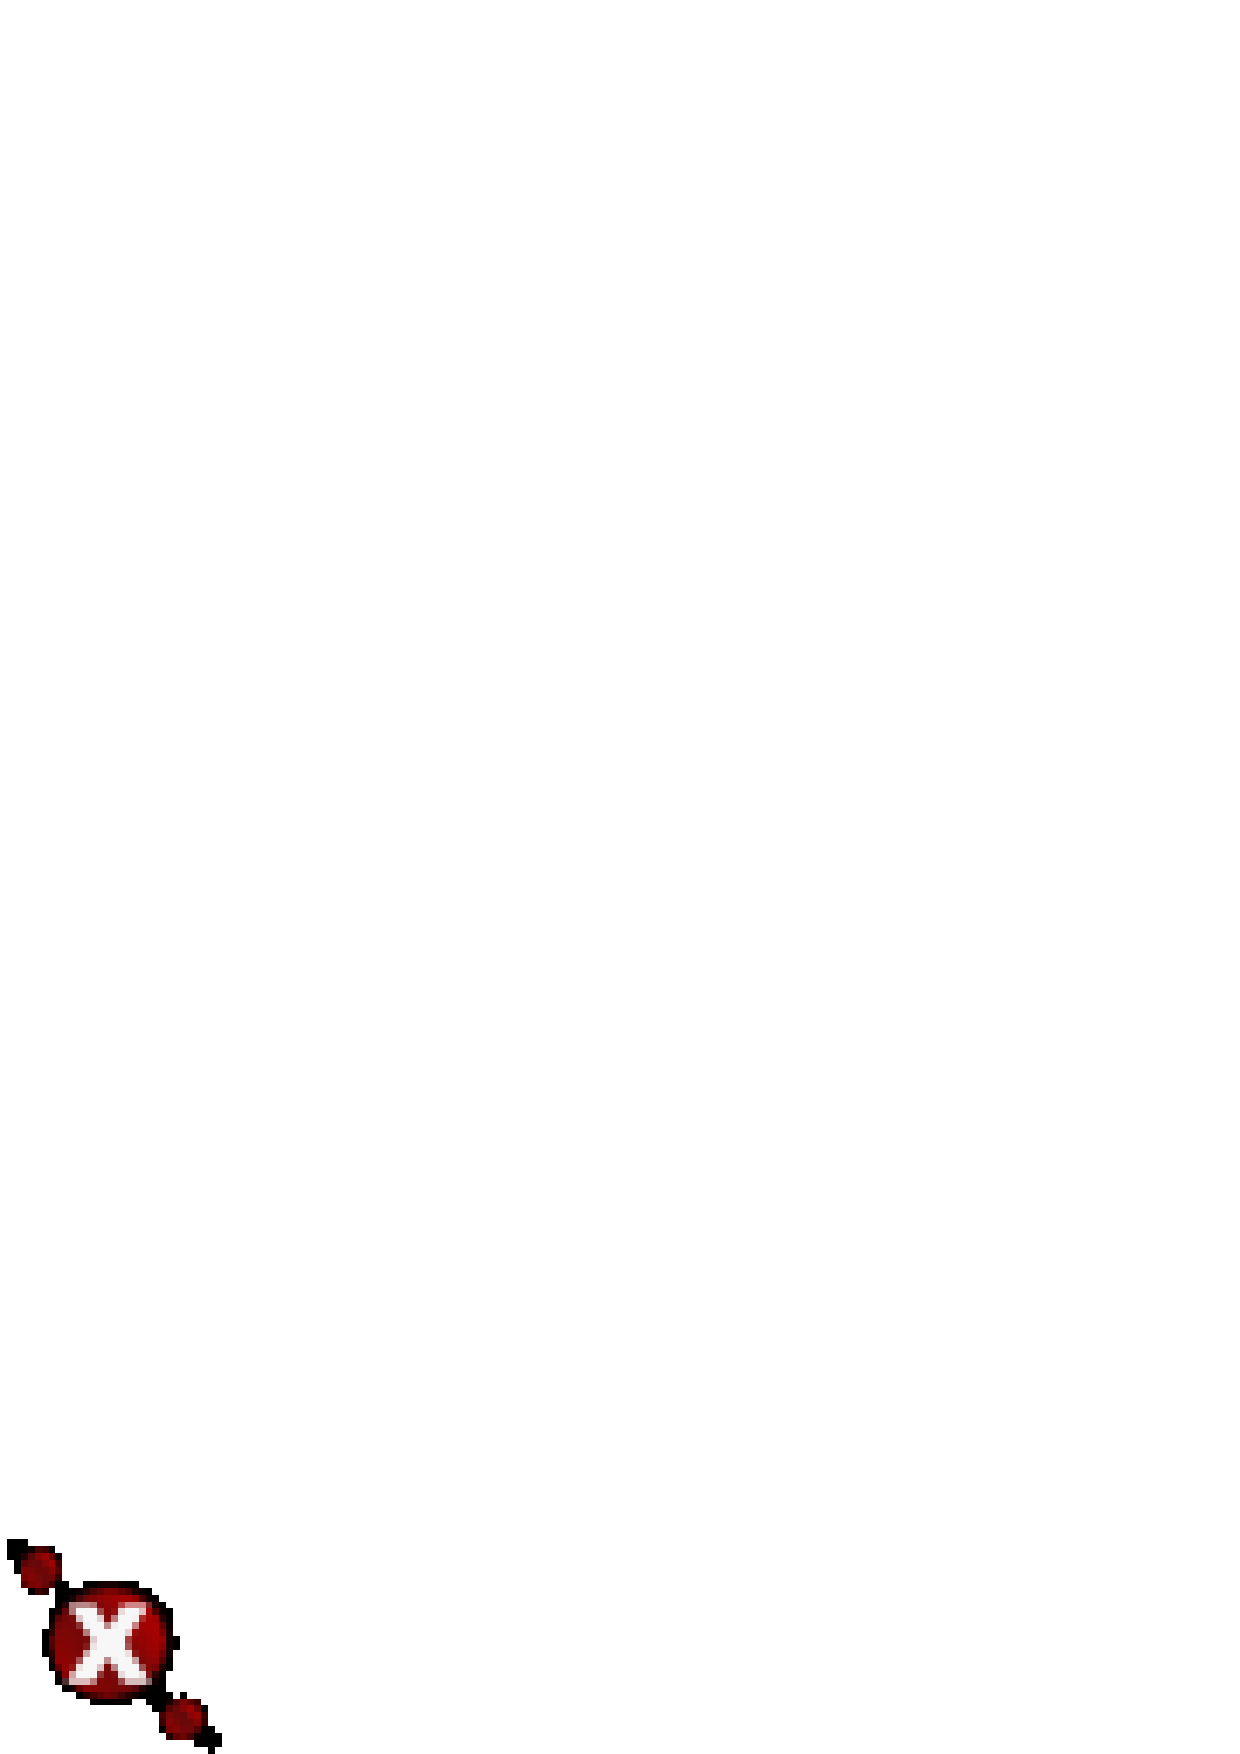
\includegraphics[width=0.7cm]{grass_delete_vertex} & Borrar vértice & Borrar un vértice de una línea existente (confirmar el vértice seleccionado con otra pulsación)\\
\hline 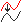
\includegraphics[width=0.7cm]{grass_move_line} & Mover elemento & Mover el contorno, línea, punto o centroide seleccionado a la nueva posición\\
\hline 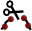
\includegraphics[width=0.7cm]{grass_split_line} & Dividir línea & Dividir una línea existente en dos partes\\
\hline 
\includegraphics[width=0.7cm]{grass_delete_line} & Borrar elemento & Borrar un contorno, línea, punto o centroide existente (confirmar el elemento seleccionado con otra pulsación)\\
\hline 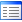
\includegraphics[width=0.7cm]{grass_edit_attributes} & Editar atributos & Editar los atributos de un elemento existente (tenga en cuenta que un elemento puede representar a más objetos espaciales, vea arriba)\\
\hline 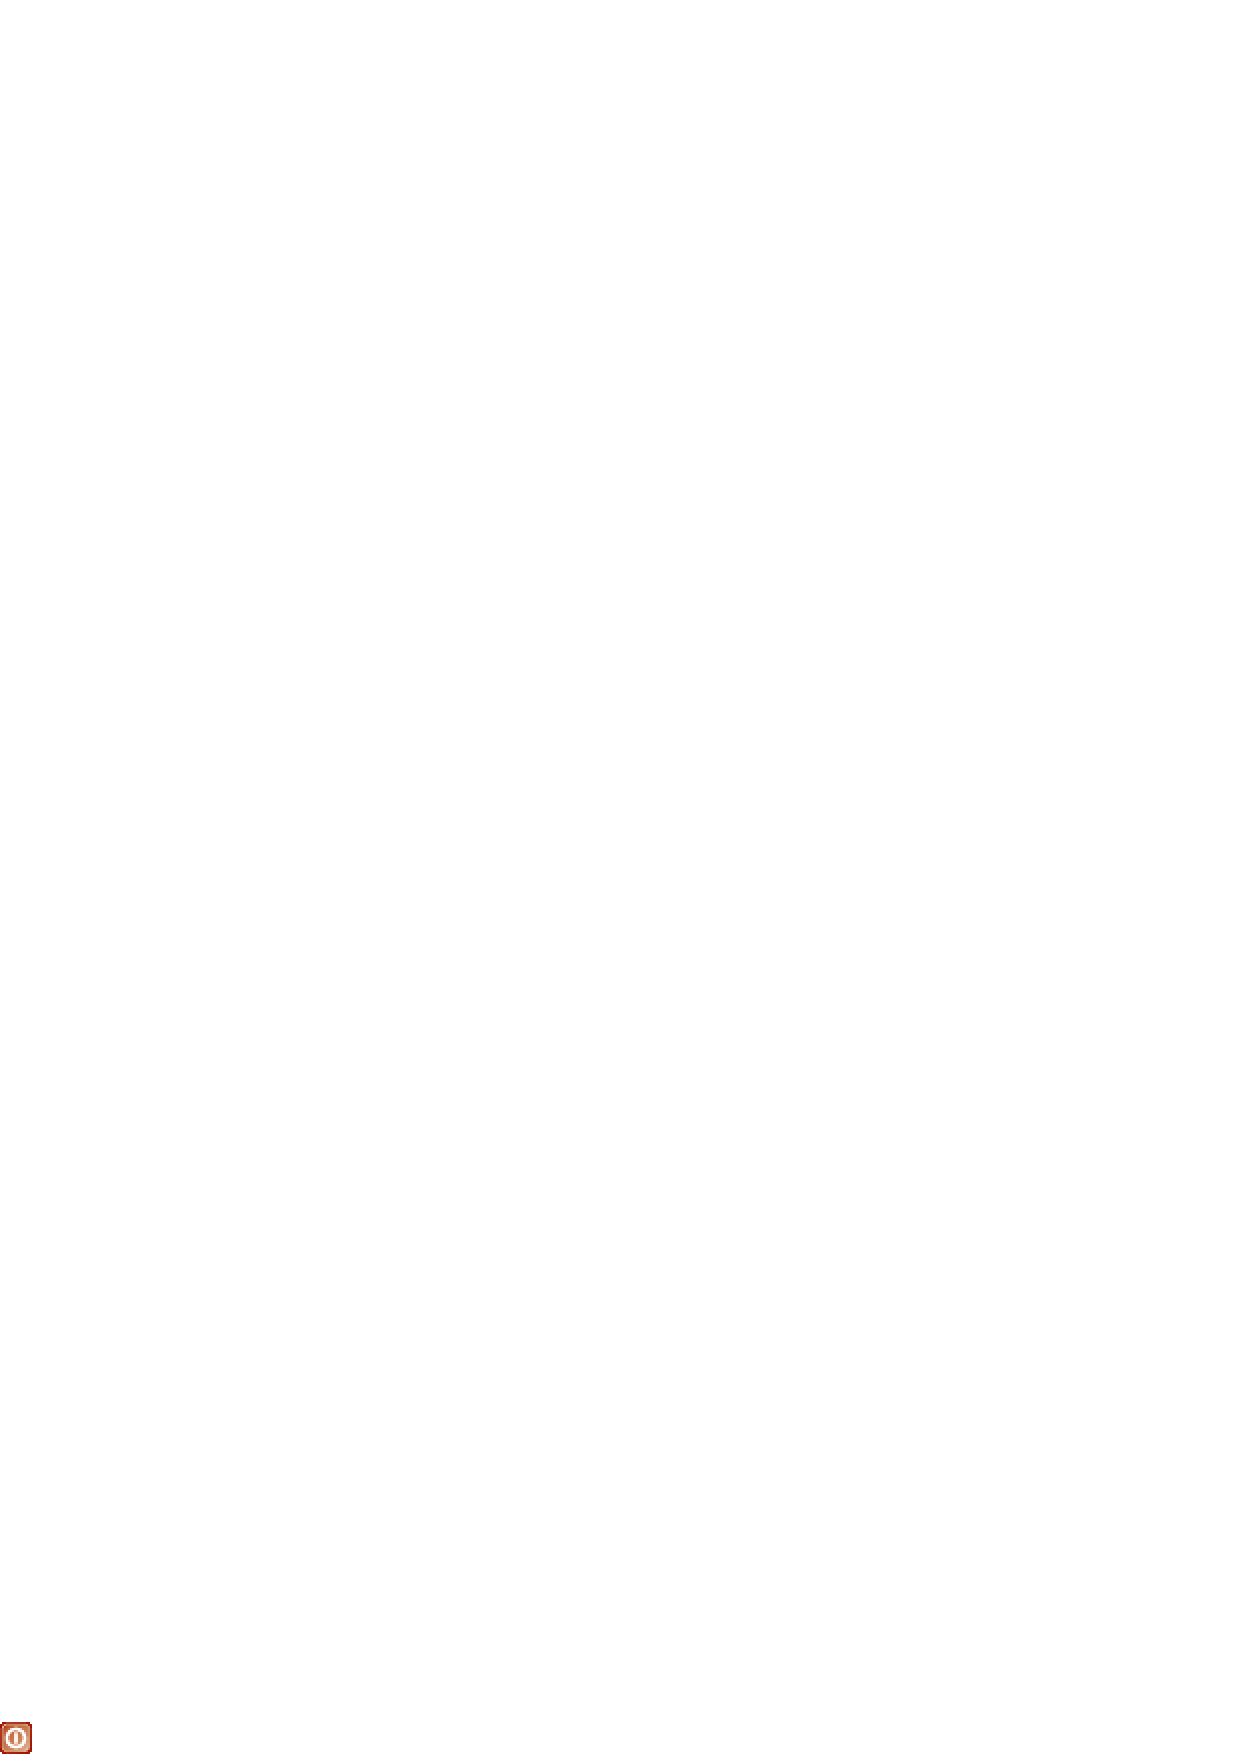
\includegraphics[width=0.7cm]{grass_close_edit} & Cerrar & Cerrar la sesión de digitalización (reconstruye la topología a continuación)\\
\hline
\end{tabular}
\end{table}

\minisec{Pestaña Categoría}\index{GRASS!category settings}

La pestaña \tab{Categoría} le permite establecer la forma en que se asignará la categoría a cada nuevo objeto espacial.

\begin{figure}[h]
 \begin{center}
  \caption{Pestaña Categoría de digitalización de GRASS \nixcaption}\label{fig:grass_digitizing_category}
  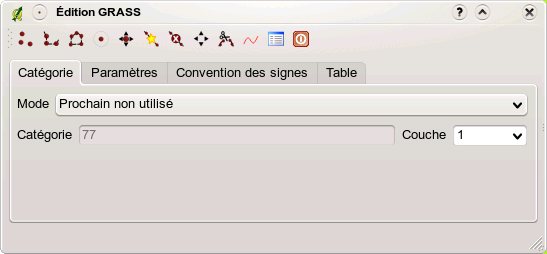
\includegraphics[clip=true,width=10cm]{grass_digitizing_category}
 \end{center}
\end{figure}

\begin{itemize}
\item \textbf{Modo}: qué valor de categoría se aplicará a los elementos de la nueva geometría.
\begin{itemize}
\item La siguiente sin usar: aplicar el siguiente valor de categoría que aún no está usado al elemento de la geometría.
\item Entrada manual: definir manualmente la categoría para el elemento de la geometría en el campo de entrada «Categoría».
\item Ninguna categoría: no aplicar ningún valor de categoría al elemento de la geometría.
Esto se usa por ejemplo para contornos de áreas, porque los valores de la categoría están conectados mediante el centroide.
\end{itemize}
\item \textbf{Categoría}: un número (ID) que se adjunta a cada elemento de la geometría 
digitalizado. Se usa para conectar cada elemento de la geometría con sus atributos.
\item \textbf{Campo (capa)} - Cada elemento de la geometría puede conectarse con varias
tablas de atributos usando diferentes capas de geometría de GRASS. El número de capa predeterminado es 1. 
\end{itemize}

\begin{Tip}\caption{\textsc{Crear «capas» adicionales de GRASS con QGIS}}
\qgistip{Si quiere añadir más capas a su conjunto de datos, simplemente añada un nuevo número en el cuadro de entrada 
«Campo (capa)» y pulse Intro. En la pestaña Tabla puede crear una nueva tabla conectada a su nueva capa.
}
\end{Tip}

\minisec{Pestaña Configuración}\label{label_settingtab}\index{GRASS!snapping
tolerance}

La pestaña \tab{Configuración} le permite establecer el autoensamblado en píxeles de la pantalla. Esto es el umbral en 
el que los nuevos puntos o finales de líneas son ensamblados de forma automática a nodos existentes. Esto ayuda a evitar 
saltos o balanceos entre contornos. El valor predeterminado es 10 píxeles.

\begin{figure}[h]
 \begin{center}
 \caption{Pestaña Configuración de digitalización de GRASS \nixcaption}\label{fig:grass_digitizing_settings}
 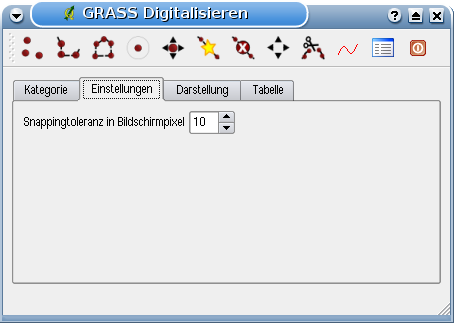
\includegraphics[clip=true,width=8cm]{grass_digitizing_settings}
 \end{center}
\end{figure}

\minisec{Pestaña Simbología}\index{GRASS!symbology settings}

La pestaña \tab{Simbología} le permite ver y establecer la simbología y la configuración del color para varios tipos de geometría y su estado topológico (ej.: contorno cerrado / abierto).

\begin{figure}[h]
 \begin{center}
 \caption{Pestaña Simbología de la digitalización de GRASS \nixcaption}\label{fig:grass_digitizing_symbology}
 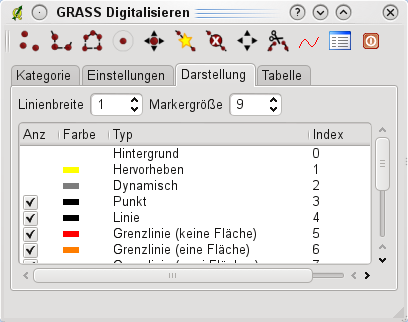
\includegraphics[clip=true,width=8cm]{grass_digitizing_symbology}
 \end{center}
\end{figure}

\minisec{Pestaña tabla} \index{GRASS!table editing}

La pestaña \tab{Tabla} proporciona información sobre la tabla de la base de datos de una «capa» dada. Aquí puede añadir 
nuevas columnas a una tabla de atributos existente o crear  una nueva tabla de base de datos para una nueva capa 
vectorial de GRASS (ver Sección 
\ref{sec:creating_new_grass_vectors}).

\begin{figure}[h]
 \begin{center}
 \caption{Pestaña tabla de la digitalización de GRASS \nixcaption}\label{fig:grass_digitizing_table}
 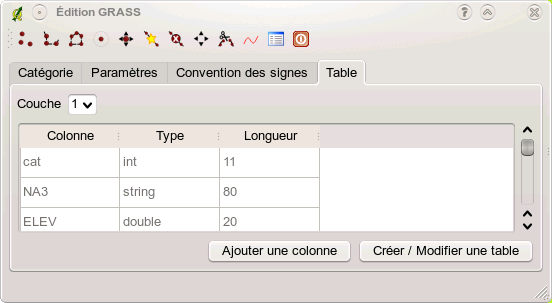
\includegraphics[clip=true,width=10cm]{grass_digitizing_table}
 \end{center}
\end{figure}

\begin{Tip}\caption{\textsc{Permisos de edición de GRASS}}\index{GRASS!edit
permissions}
\qgistip{Tiene que ser el propietario del \filename{DIRECTORIO DE MAPAS} de GRASS que quiera editar. Es imposible editar 
capas de datos en \filename{DIRECTORIOS DE MAPAS} que no sean suyos, incluso si tiene permiso de escritura.
}
\end{Tip} 

\subsection{La herramienta Región de GRASS}\label{sec:grass_region}\index{GRASS!region}

La definición de la región (establecer una ventana de trabajo espacial) en GRASS es importante para trabajar con capas
ráster. El análisis vectorial no está limitado de forma predeterminada a ninguna región definida. Todos los ráster de nueva 
creación tienen la extensión espacial y resolución de la región actual, no importa cuál sea su extensión y resolución original. La región actual de GRASS se guarda en el archivo \filename{\$LOCATION/\$MAPSET/WIND}, y define los límites Norte, Sur, Este y Oeste, número de columnas y filas y la resolución espacial horizontal y vertical.

Se puede activar/descactivar la visualización de la región de GRASS en la vista del mapa de QGIS usando el botón 
\toolbtntwo{grass_region}{Mostrar región actual de GRASS}. \index{GRASS!region!display}.

Con el icono \toolbtntwo{grass_region_edit}{Editar la región actual de GRASS} puede abrir un diálogo en el que puede 
cambiar la región actual y la simbología del rectángulo de la región de GRASS en la vista del mapa de QGIS. Escriba
los nuevos límites y resolución y pulse \button{Aceptar}. Cuando se está ejecutando la herramienta también es posible 
seleccionar una nueva región de forma interactiva con el ratón sobre el lienzo de QGIS.
Para ello pulse con el botón 
izquierdo del ratón en el lienzo de QGIS, abra un rectángulo, cierrelo usando el botón izquierdo de nuevo y pulse 
\button{Aceptar}.\index{GRASS!region!editing}
El módulo de GRASS \filename{g.region} proporciona muchos más parámetros para definir una extensión y resolución adecuadas
de la región para su análisis ráster. Puede usar estos parámetros con la Caja de herramientas de GRASS, descrita en la Sección 
\ref{subsec:grass_toolbox}.

\subsection{La Caja de herramientas de GRASS}\label{subsec:grass_toolbox}\index{GRASS!toolbox}

El cuadro \toolbtntwo{grass_tools}{Abrir herramientas de GRASS} proporciona funciones de los módulos de GRASS para trabajar 
con datos dentro de una \filename{LOCALIZACIÓN} y \filename{DIRECTORIO DE MAPAS} seleccionados. Para usar la caja 
de herramientas de GRASS necesita abrir una \filename{LOCALIZACIÓN} y un \filename{DIRECTORIO DE MAPAS} en el que 
tenga permiso de escritura (normalmente lo tendrá si creó el \filename{DIRECTORIO DE MAPAS}). Esto es necesario porque 
se tienen que escribir nuevas capas ráster o vectoriales en la \filename{LOCALIZACIÓN} y el \filename{DIRECTORIO DE MAPAS} 
seleccionados creadas durante el análisis.

\subsubsection{Trabajar con módulos de GRASS}\index{GRASS!toolbox}

\begin{figure}[h]
\centering
\caption{Caja de herramientas de GRASS y Lista de búsqueda de módulos \nixcaption}\label{fig:grass_modules}
   \subfigure[Árbol de módulos] {\label{subfig:grass_module_tree}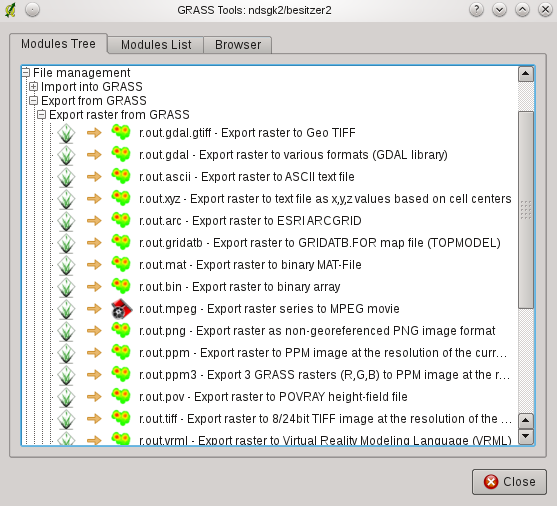
\includegraphics[clip=true, width=0.4\textwidth]{grass_toolbox_moduletree}}\goodgap
   \subfigure[Lista de búsqueda de módulos] {\label{subfig:grass_module_list}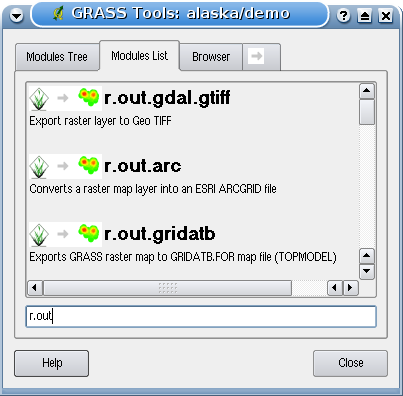
\includegraphics[clip=true, width=0.4\textwidth]{grass_toolbox_modulelist}}
\end{figure}

La consola de GRASS dentro de la caja de herramientas de GRASS proporciona acceso a casi todos (más de 300) los módulos de
 GRASS en modo línea de órdenes. Para ofrecer un entorno de trabajo más amigable, unos 200 de los módulos y funcionalidades 
disponibles de GRASS también se proporcionan mediante diáologos gráficos. Estos diálogos están agrupados en bloques temáticos, 
pero también se pueden buscar. Encontrará una lista completa de los módulos de GRASS disponibles en la versión de QGIS \CURRENT
en el apédice \ref{appdx_grass_toolbox_modules}. También es posible personalizar el contenido de la caja de herramientas de 
GRASS. Esto se describe en la Sección \ref{sec:toolbox-customizing}.

Como se muestra en la Figura \ref{fig:grass_modules}, puede buscar el módulo adecuado usando las pestañas \tab{Árbol de módulos} o \tab{Lista de módulos}.

Al pulsar en el icono de un módulo se añadirá una nueva pestaña a su caja de herramientas que proporciona tres 
nuevas subpestañas \tab{Opciones}, \tab{Salida} y \tab{Manual}. En la Figura \ref{fig:grass_module_dialog} se 
ve un ejemplo para el módulo de GRASS \filename{v.buffer}.

\begin{figure}[h]
\centering
\caption{Diálogos de módulo de la caja de herramientas de GRASS \nixcaption}\label{fig:grass_module_dialog}
   \subfigure[Opciones del módulo] {\label{subfig:grass_module_option}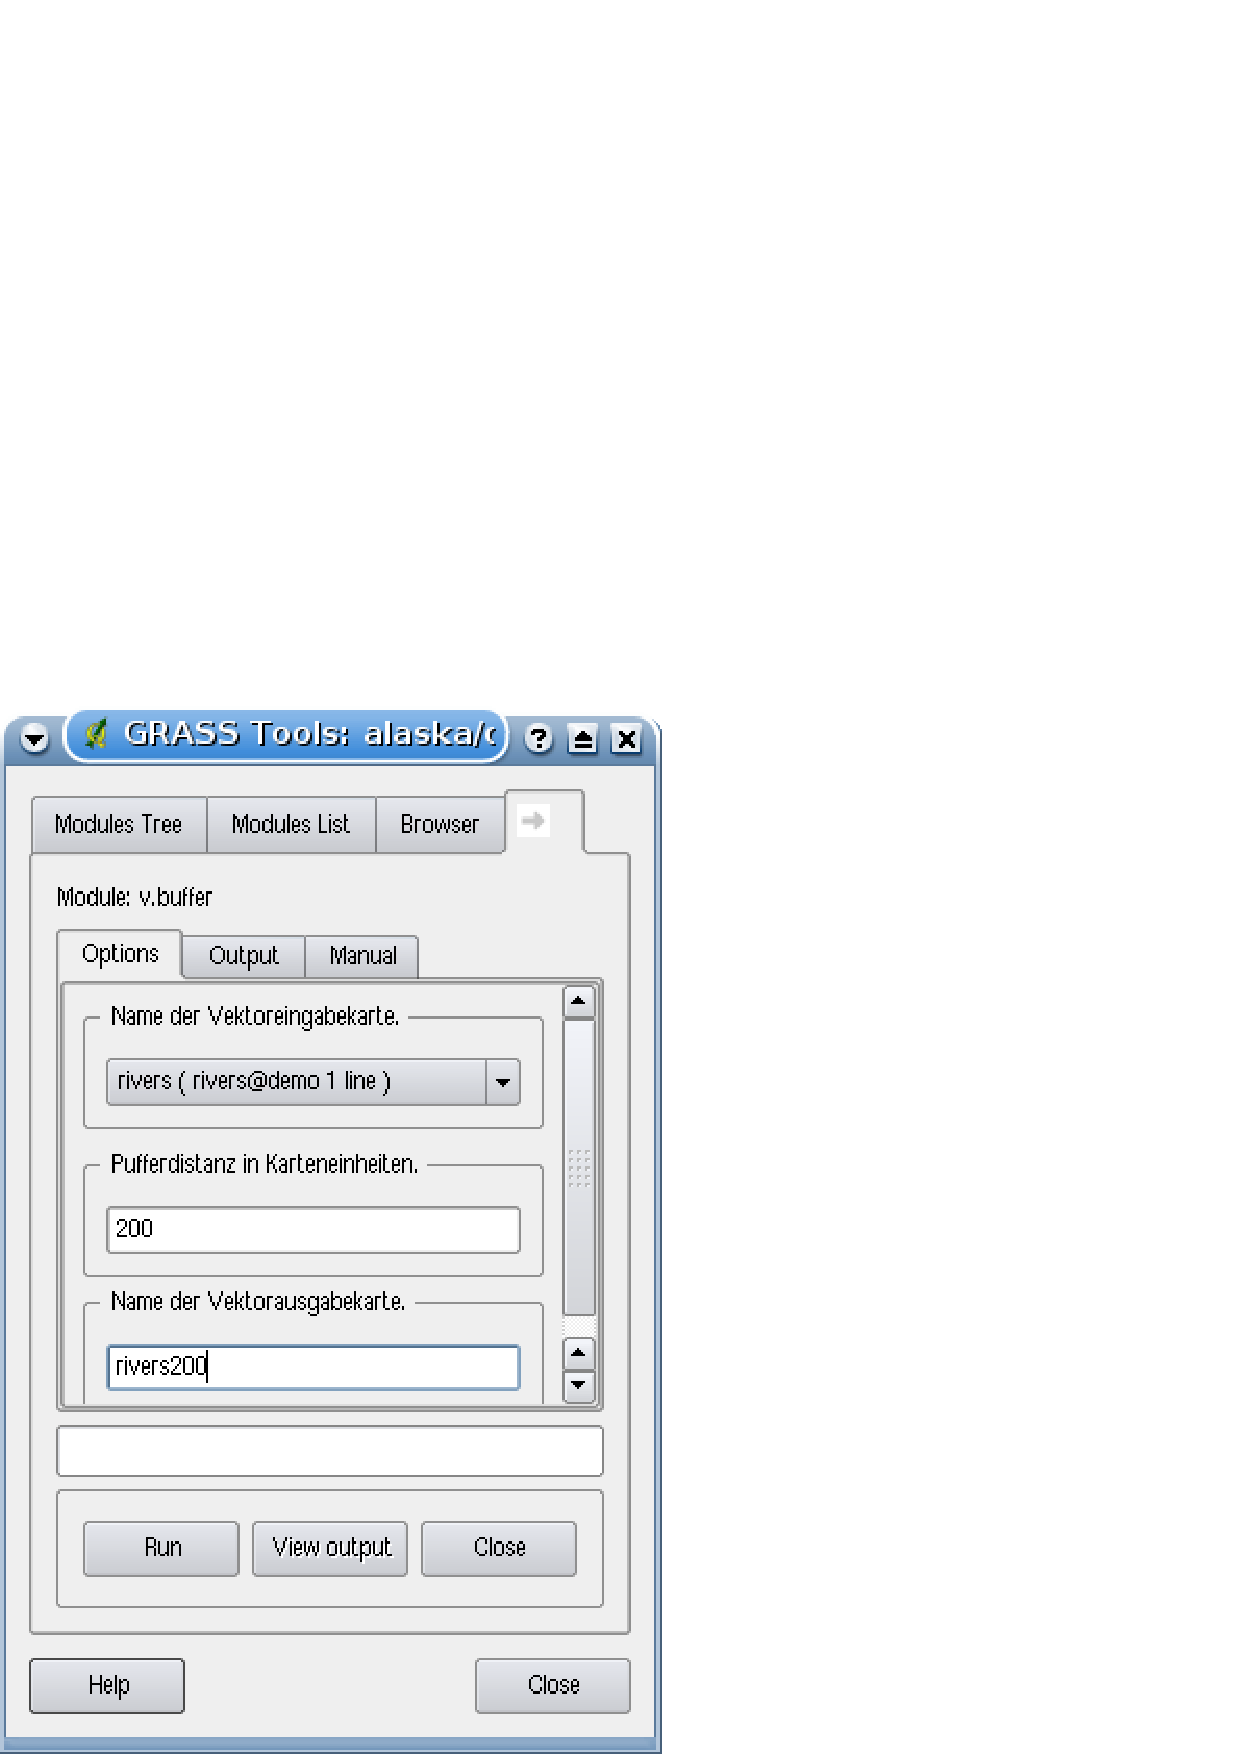
\includegraphics[clip=true, width=0.3\textwidth]{grass_module_option}}\goodgap
   \subfigure[Salida del módulo] {\label{subfig:grass_module_output}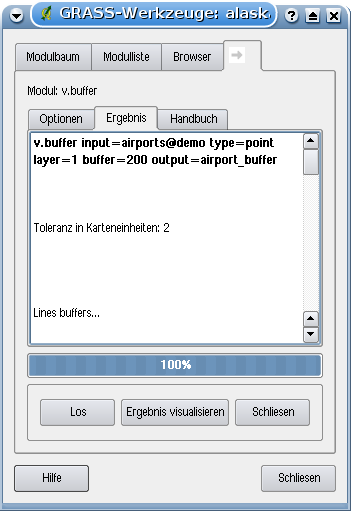
\includegraphics[clip=true, width=0.3\textwidth]{grass_module_output}}\goodgap
   \subfigure[Manual del módulo] {\label{subfig:grass_module_manual}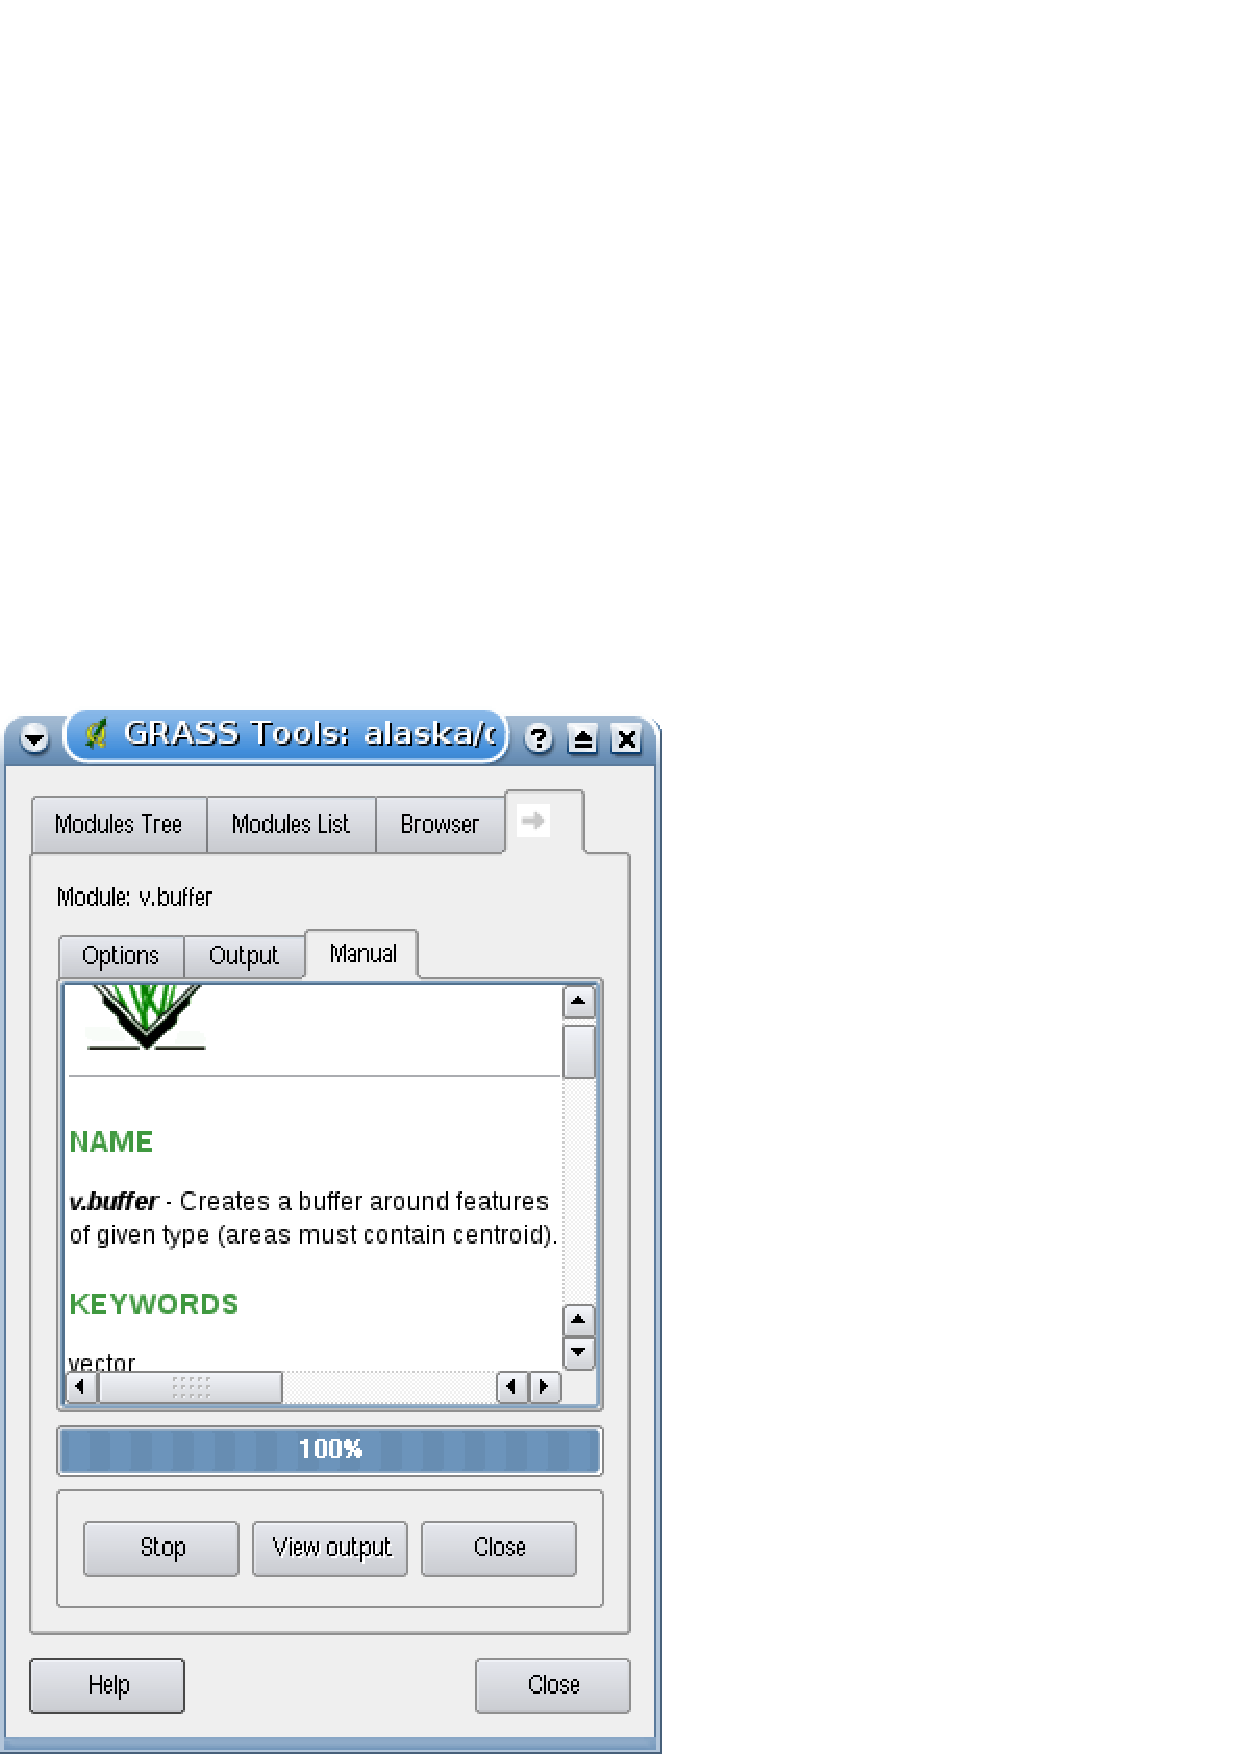
\includegraphics[clip=true, width=0.3\textwidth]{grass_module_manual}}
\end{figure}

\minisec{Opciones}

La pestaña \tab{Opciones} proporciona un diálogo simplificado del módulo en el que normalmente puede seleccionar una 
capa ráster o vectorial visualizada en el lienzo de QGIS e introducir otros parámetros específicos del módulo seleccionado 
para ejecutarlo. Los parámetros del módulo proporcionados a menudo no están completos, para mantener despejado el diálogo.
Si quiere usar más parámetros y opciones del módulo, necesitará iniciar la consola de GRASS y ejecutar el módulo en línea
de órdenes.

\minisec{Salida}

La pestaña \tab{Salida} proporciona información sobre el estado de salida del módulo. Cuando se pulsa el botón \button{Ejecutar}, 
el módulo pasa a la pestaña \tab{Salida} y verá información sobre el proceso de análisis. Si todo va bien, al final verá 
el mensaje \usertext{Finalizado correctamente}.

\minisec{Manual}

La pestaña \tab{Manual} muesta la página de ayuda HTML del módulo de GRASS. Puede usarla para comprobar más parámetros y 
opciones del módulo o para obtener un conocimiento mayor sobre el objetivo del módulo. Al final de la página de cada módulo 
hay más enlaces al \filename{Índice principal de la Ayuda}, al \filename{Índice temático} y al \filename{Índice completo}. 
Estos enlaces proporcionan la misma información que si usa el módulo \filename{g.manual} 

\begin{Tip}\caption{\textsc{Mostrar resultados inmediatamente}}\index{GRASS!display results}
\qgistip{Si quiere mostrar los resultados de sus cálculos inmediatamente en el lienzo de su mapa, puede usar el botón «Ver salida» de la parte inferior de la pestaña del módulo.
}
\end{Tip} 

\subsubsection{Trabajar con el explorador de LOCALIZACIONES de GRASS} \index{GRASS!toolbox!Browser}

Otra función útil dentro de la Caja de herramientas de GRASS es el explorador de 
\filename{LOCALIZACIONES} de GRASS. En la Figura~\ref{fig:grass_mapset_browser} puede ver la \filename{LOCALIZACIÓN} actual de trabajo con sus \filename{DIRECTORIOS DE MAPAS}.

En la ventana de la izquierda del explorador puede navegar por todos sus \filename{DIRECTORIOS DE MAPAS} 
dentro de la \filename{LOCALIZACIÓN} actual. La parte derecha de la ventana del explorador muestra alguna metainformación 
de las capas ráster o vectoriales seleccionadas, por ejemplo la resolución, cuadro delimitador, fuente de datos, tabla 
de atributos conectada para datos vectoriales y un historial de órdenes.

\begin{figure}[h]
 \begin{center}
 \caption{Explorador de LOCALIZACIONES de GRASS \nixcaption}\label{fig:grass_mapset_browser}
 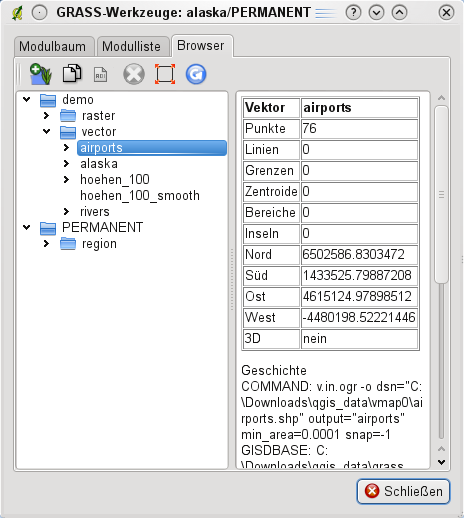
\includegraphics[clip=true,width=10cm]{grass_mapset_browser}
 \end{center}
\end{figure}

La barra de herramientas que hay dentro de la pestaña \tab{Explorador} la proporciona las siguientes herramientas para administrar la \filename{LOCALIZACIÓN} seleccionada:

\begin{itemize}
\item \toolboxtwo{grass_add_map}{Añadir el mapa seleccionado a la vista del mapa}
\item \toolboxtwo{grass_copy_map}{Copiar el mapa seleccionado}
\item \toolboxtwo{grass_rename_map}{Cambiar el nombre al mapa seleccionado}
\item \toolboxtwo{grass_delete_map}{Borrar el mapa seleccionado}
\item \toolboxtwo{grass_set_region}{Establecer la región actual al mapa seleccionado}
\item \toolboxtwo{grass_refresh}{Actualizar la ventana del explorador}
\end{itemize}

\toolboxtwo{grass_rename_map}{Cambiar el nombre al mapa seleccionado} y 
\toolboxtwo{grass_delete_map}{Borrar el mapa seleccionado} 
sólo funcionan con mapas que estén dentro de su \filename{DIRECTORIO DE MAPAS} actualmente seleccionado. Todas las 
demás herramientas también funcionan con capas ráster y vectoriales de otros \filename{DIRECTORIOS DE MAPAS}.

\subsubsection{Personalizar la Caja de herramientas de GRASS} \index{GRASS!toolbox!customize}
\label{sec:toolbox-customizing}

Casi todos los módulos de GRASS se pueden añadir a la caja de herramientas de GRASS. Se proporciona una interfaz XML para 
analizar los sencillos archivos XML que configuran el aspecto y los parámetros de los módulos dentro de la caja de herramientas. 

Un ejemplo de archivo XML para generar el módulo \usertext{v.buffer} (v.buffer.qgm) 
tiene este aspecto:
\begin{verbatim}
<?xml version="1.0" encoding="UTF-8"?>
<!DOCTYPE qgisgrassmodule SYSTEM "http://mrcc.com/qgisgrassmodule.dtd">

<qgisgrassmodule label="Vector buffer" module="v.buffer">
        <option key="input" typeoption="type" layeroption="layer" />
        <option key="buffer"/>
        <option key="output" />
</qgisgrassmodule>
\end{verbatim}

El analizador lee esta definición y crea una pestaña nueva dentro de la caja de herramientas cuando selecciona el 
módulo. Se puede encontrar una descripción más detallada sobre cómo añadir nuevos módulos, cambiar los grupos de 
módulos, etc. en el wiki de QGIS en \\
\url{http://wiki.qgis.org/qgiswiki/Adding\_New\_Tools\_to\_the\_GRASS\_Toolbox}.

